\documentclass[12pt,oneside]{article}

%%%%%%%%%%%%%%%%%%%%%%%%%%%%
%%   Zusaetzliche Pakete  %%
%%%%%%%%%%%%%%%%%%%%%%%%%%%%
\usepackage{acronym}
\usepackage{enumerate}  
\usepackage{a4wide}
\usepackage{fancyhdr}
\usepackage{graphicx}
\usepackage{palatino}
\usepackage{blindtext}
\usepackage{multirow}
\usepackage{amsmath}
\usepackage{amssymb}
\usepackage{float}
\usepackage{algpseudocode}

\usepackage[ruled,longend]{algorithm2e}
\usepackage{float}
\usepackage{url}
\usepackage{pdfpages}
\usepackage{booktabs}


% für englische Arbeiten "ngerman" durch "english" ersetzen
\usepackage[english]{babel}

\usepackage[T1]{fontenc}
\usepackage[utf8]{inputenc}
\usepackage[utf8]{inputenc}

%Hervorherbung für Links entfernen
%\usepackage[bookmarks]{hyperref}
\usepackage[bookmarks, pdfborder={0 0 0}]{hyperref}

\usepackage[justification=centering]{caption}
\usepackage{csquotes}


%%%%%%%%%%%%%%%%%%%%%%%%%%%
%% Define line spacing   %%
%%%%%%%%%%%%%%%%%%%%%%%%%%%
\usepackage{setspace}
\setlength{\parindent}{0em}
\setlength{\parskip}{0.5em}

\usepackage{enumitem}
\setlist[itemize]{topsep=0pt, partopsep=0pt, itemsep=-1pt, parsep=3pt}
\setlist[enumerate]{topsep=0pt, partopsep=0pt, itemsep=-1pt, parsep=3pt}

\setlist[1]{topsep=2pt, itemsep=3pt, parsep=4pt}
\setlist[2]{topsep=0pt, itemsep=1pt, parsep=2pt}
\setlist[3]{topsep=-1pt, noitemsep}

% Formating the page
\usepackage{microtype}
% Do not allow single lines at the end of a page
\clubpenalty = 10000
% Do not allow single lines at the beginning of a page
\widowpenalty = 10000 \displaywidowpenalty = 10000


%%%%%%%%%%%%%%%%%%%%%%%%%%%
%$ APA Style für Bibtex  %%
%%%%%%%%%%%%%%%%%%%%%%%%%%%
\usepackage[style=numeric,natbib=true,backend=biber, sorting=none]{biblatex}


\DefineBibliographyStrings{english}{
  bibliography = {References},
}
\bibliography{citations.bib}

% Note: The following commands need the "url" package
\setcounter{biburlnumpenalty}{100}
\setcounter{biburlucpenalty}{100}
\setcounter{biburllcpenalty}{100}

% This will count equasions 
\counterwithin{equation}{section}


%%%%%%%%%%%%%%%%%%%%%%%%%%%%%%
%% Definition der Kopfzeile %%
%%%%%%%%%%%%%%%%%%%%%%%%%%%%%%

\pagestyle{fancy}
\fancyhf{}
\cfoot{\thepage}
\setlength{\headheight}{16pt}


%%%%%%%%%%%%%%%%%%%%%%%%%%%%%%%%%%%%%%%%%%%%%%%%%%%%%
%%  Definition des Deckblattes und der Titelseite  %%
%%  Do not edit                                    %%
%%%%%%%%%%%%%%%%%%%%%%%%%%%%%%%%%%%%%%%%%%%%%%%%%%%%%

\newcommand{\UDOTitle}[9]{

  \thispagestyle{empty}
  
\includegraphics[width=3in]{abbildungen/tud_logo_rgb.jpg}
  \vspace*{\stretch{1}}
  \\
  {\parindent0cm
  \rule{\linewidth}{.1ex}}
  \begin{flushright}
    \vspace*{\stretch{1}}
    \sffamily\bfseries\Huge
    #1\\
    \vspace*{\stretch{1}}
    \sffamily\bfseries\large
    #2\\
    \vspace*{\stretch{1}}
  \end{flushright}
  \rule{\linewidth}{.1ex}

  \vspace*{\stretch{1}}
  \begin{center}

    \vspace*{\stretch{1}}
    \large #5\\

    \vspace*{\stretch{1}}
    \large #3\\ 
    \large  #8 \\ 
    \large  #9 \\ 

    \vspace*{\stretch{1}}
    \large  #6 -- #7

    \vspace*{\stretch{2}}
    \end{center}
}


%%%%%%%%%%%%%%%%%%%%%%%%%%%%
%%  Beginn des Dokuments  %%
%%%%%%%%%%%%%%%%%%%%%%%%%%%%
\setcounter{tocdepth}{2}

\begin{document}
\sloppy

  \UDOTitle
      {Integrating Logical Constraints in One-Class Graph Neural Networks for Anomaly Detection}                            % Titel der Arbeit
      {Anastasiia Romanenko}                           % Vor- und Nachname des Autors
      {242436}                                     % Matrikelnummer des Autors
      {Bachelor Data Science}     % Studiengang
      {Bachelorarbeit}   % Art der Arbeit
      {dd.mm.yyyy}                                  % Tag der Anmeldung
      {dd.mm.yyyy}                                  % Tag der Abgabe
      {Prof. Dr. Emmanuel Müller}                % Name des Erstgutachters
      {Tim Katzke}                                        % Name des Zweitgutachters
      
  \clearpage


%%%%%%%%%%%%%%%%%%%%%%%%%%%%
%%  Zusammenfassung   %%
%%%%%%%%%%%%%%%%%%%%%%%%%%%%
\pagenumbering{Roman} 
    \setcounter{page}{1}
    

\lhead{}

\tableofcontents
\thispagestyle{empty}
\clearpage

\pagenumbering{Roman} 
    \setcounter{page}{3}
    
\addcontentsline{toc}{section}{\listfigurename}
{%
   	\let\oldnumberline\numberline%
   	\renewcommand{\numberline}{\figurename~\oldnumberline}%
   	\listoffigures%
}
\clearpage
    
\addcontentsline{toc}{section}{\listtablename}
{%
   	\let\oldnumberline\numberline%
   	\renewcommand{\numberline}{\tablename~\oldnumberline}%
   	\listoftables%
}
\clearpage


% Formelverzeichnis können an dieser Stelle sinnvolle Ergänzungen sein.


%%%%%%%%%%%%%%%%%%%%%%%%%%%%
%%  Einstellungen  %%
%%%%%%%%%%%%%%%%%%%%%%%%%%%%
\cleardoublepage
\pagenumbering{arabic}  
    \setcounter{page}{1}
\lhead{\nouppercase{\leftmark}}


\section{Introduction and Motivation}
\label{sec:introduction}

Anomaly detection \cite{chandola2009anomaly} is a fundamental task in data analysis, with applications ranging from fraud detection in financial networks and intrusion detection in cybersecurity to identifying unusual molecular structures in drug discovery. As data in many real-world domains is naturally represented as graphs---where entities are nodes and their relationships are edges---there is a growing need for methods that can detect anomalies in graph-structured data.

Graph neural networks (GNNs) \cite{kipf2017gcn} have emerged as a powerful class of models for learning on graphs. Among them, one-class GNNs, particularly the One-Class Graph Isomorphism Network (OCGIN) \cite{ocgin}, have shown promise for anomaly detection. OCGIN extends the Deep SVDD framework \cite{pmlr-v80-ruff18a} to graph data by learning to map node or graph embeddings close to a center in the embedding space, under the assumption that normal samples cluster together while anomalies lie farther away.

However, this one-class formulation comes with known challenges. The model may converge to a trivial solution where all embeddings collapse to the center---a phenomenon called hypersphere collapse. Furthermore, the standard OCGIN objective is purely data-driven and does not incorporate any prior knowledge about what constitutes normal or anomalous structure in the data.

Logical constraints have recently gained attention as a way to inject domain knowledge into deep learning models \cite{xu2018semanticloss}. By formalizing prior knowledge as logical rules and making them differentiable, one can guide the learning process toward solutions that are both data-driven and logically consistent. This approach has been shown to improve performance, reduce data requirements, and enhance interpretability \cite{Giunchiglia_2022}, \cite{stoian2024realisticsyntheticdataconstraining} .

\subsection{Research Question and Contributions}

In this thesis, we propose to combine these two lines of research by integrating logical constraints into one-class graph neural networks for anomaly detection. More specifically, we address the following research question: Can logical constraints extracted from structural graph features improve the representations learned by one-class GNNs for anomaly detection?

Our approach consists of three main components. First, we extract logical rules from graph data by training a decision tree \cite{breiman1984cart} on structural continious features (e.g., node attributes, node degree) and converting each root-to-leaf path into a conjunctive rule. For categorical node attribute features we train a Logic Tensor Network \cite{Badreddine_2022} and extract logical rules. Second, we make these rules differentiable using two alternative strategies---a fuzzy logic-based evaluation \cite{fuzzylogicbook} [p. 9-12], and a proposed in this work distance-based scoring that considers the margin of samples to decision boundaries. Third, we integrate the resulting constraint values into the OCGIN loss function through three distinct strategies: additive penalty, weighting, and suppression.

We further distinguish between two inference paradigms: in loss-only models, constraints influence only the training objective, while in constraint-aware models, they also affect the anomaly score at inference time. This allows us to isolate whether the improvements come from regularized training or from direct constraint-based scoring.

We evaluate our proposed methods on a diverse collection of over 13 graph datasets spanning citation networks, co-authorship graphs, molecular structures, protein graphs, and computer vision tasks, at both the node and graph levels. Through extensive hyperparameter tuning, we compare each logic-enhanced variant against its baseline OCGIN counterpart.

\subsection{Structure Overview}

The remainder of this thesis is organized as follows. Chapter~\ref{sec:background} provides the theoretical background on graph theory, neural networks, graph anomaly detection with OCGIN, and logical constraints in deep learning. Chapter~\ref{sec:methodology} describes our proposed methodology in detail, including the motivation and functions of the constraint generation pipeline, differentiable constraint handlers, and loss integration strategies. Chapter~\ref{sec:evaluation} presents the experimental setup, datasets, hyperparameter configurations, and results. Finally, Chapter~\ref{sec:conclusion} concludes the thesis and discusses directions for future work.


\clearpage
\section{Theoretical Background}
\label{sec:background}

In this chapter, we will provide the theoretical background on anomaly detection with graph neural networks and on research in deep learning with logical constraints. First, we introduce graph theory. Then, we discuss the theoretical foundations of neural networks and their evaluation methods. Next, we combine this knowledge and describe an existing graph anomaly detection framework—the One-Class Graph Isomorphism Network. Afterwards, we provide an overview of logical constraints in deep learning and decision trees.

\subsection{Graph Theory}

A graph is an abstract data structure that captures entities and the relationships between them \cite{west2001graph}. Formally, a graph is defined as a pair
\begin{equation}
G = (V, E),
\end{equation}
where $V$ is a set of vertices (or nodes), and $E$ is a set of edges. In an undirected graph, each edge is an unordered pair $\{x, y\}$ with $x, y \in V$.

If two vertices are connected by an edge, they are called neighbors (or adjacent). Formally, given $x, y \in V$ and $\{x, y\} \in E$, $x$ and $y$ are neighbors. Two edges $e, f \in E$ are said to be adjacent if they share a common endpoint (node).

The neighborhood of a vertex $y \in V$ is given by
\begin{equation}
N(y) = \{ x \in V \mid \{x, y\} \in E \}.
\end{equation}

The number of neighbors of a node is called the degree of the vertex, denoted by $|N(y)|$. A vertex with degree zero is called an isolated vertex.

\begin{minipage}{\textwidth}
    \centering
    \begin{minipage}[t]{0.55\textwidth}
        \centering
        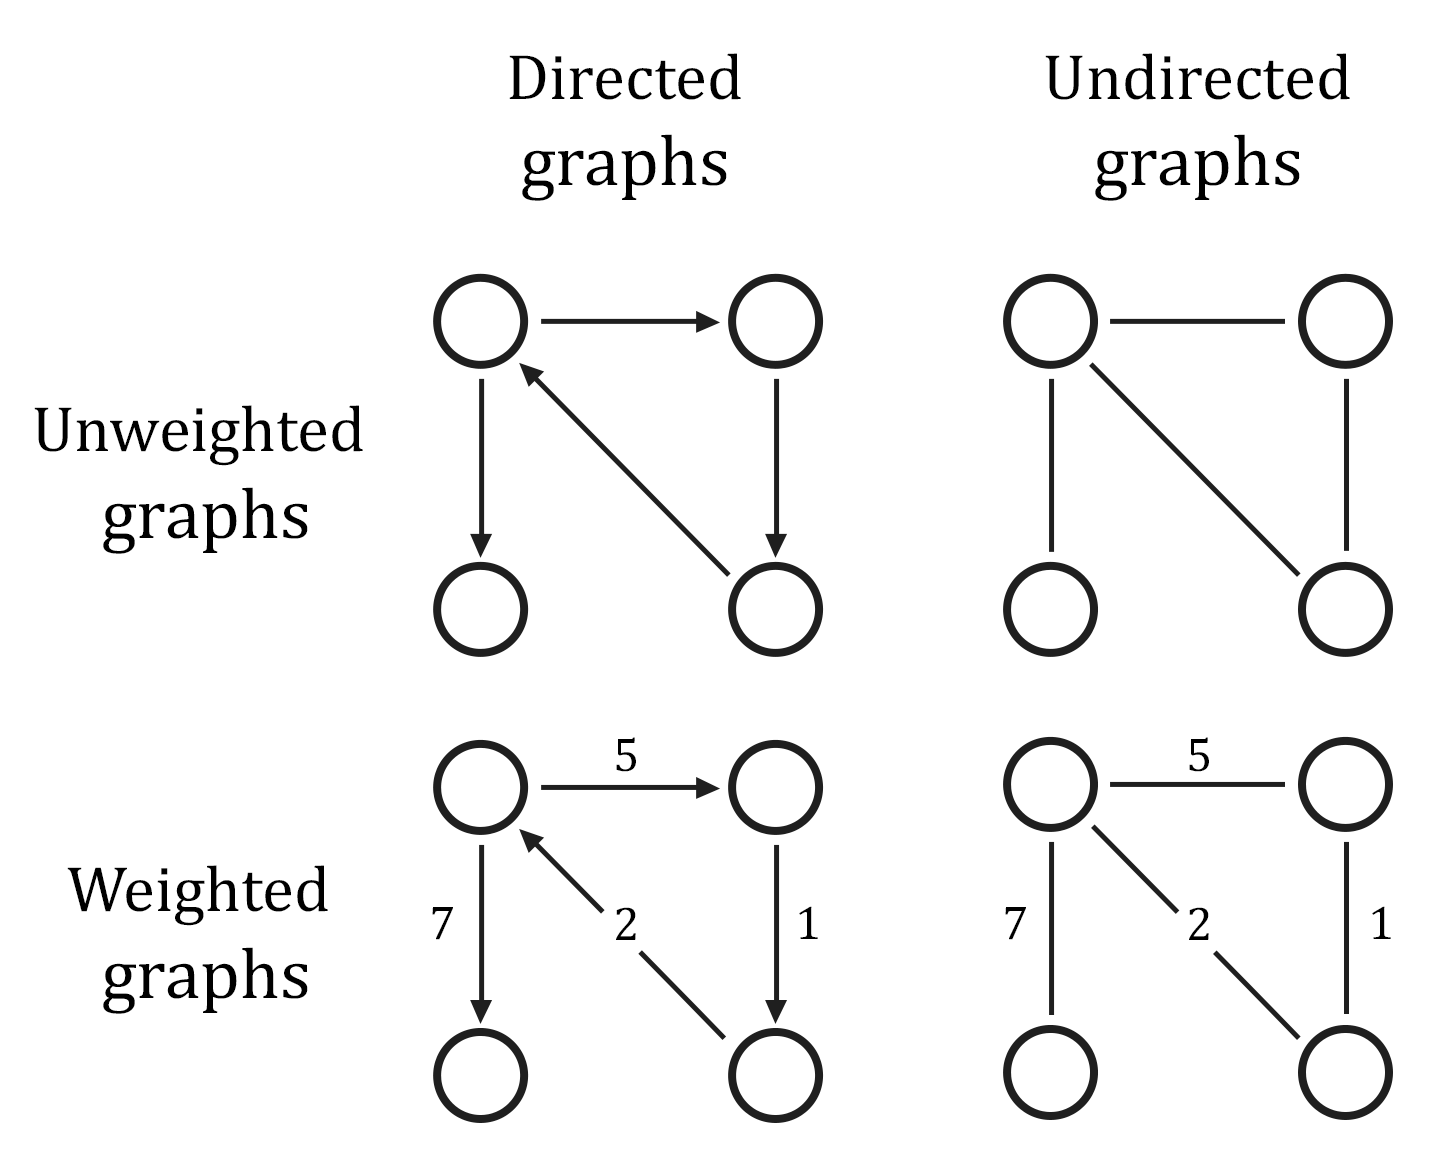
\includegraphics[width=\linewidth]{plots/graph_types.png}
        \captionof{figure}{Types of graphs}
        \label{fig:graph_types}
    \end{minipage}
    \begin{minipage}[t]{0.44\textwidth}
        \centering
        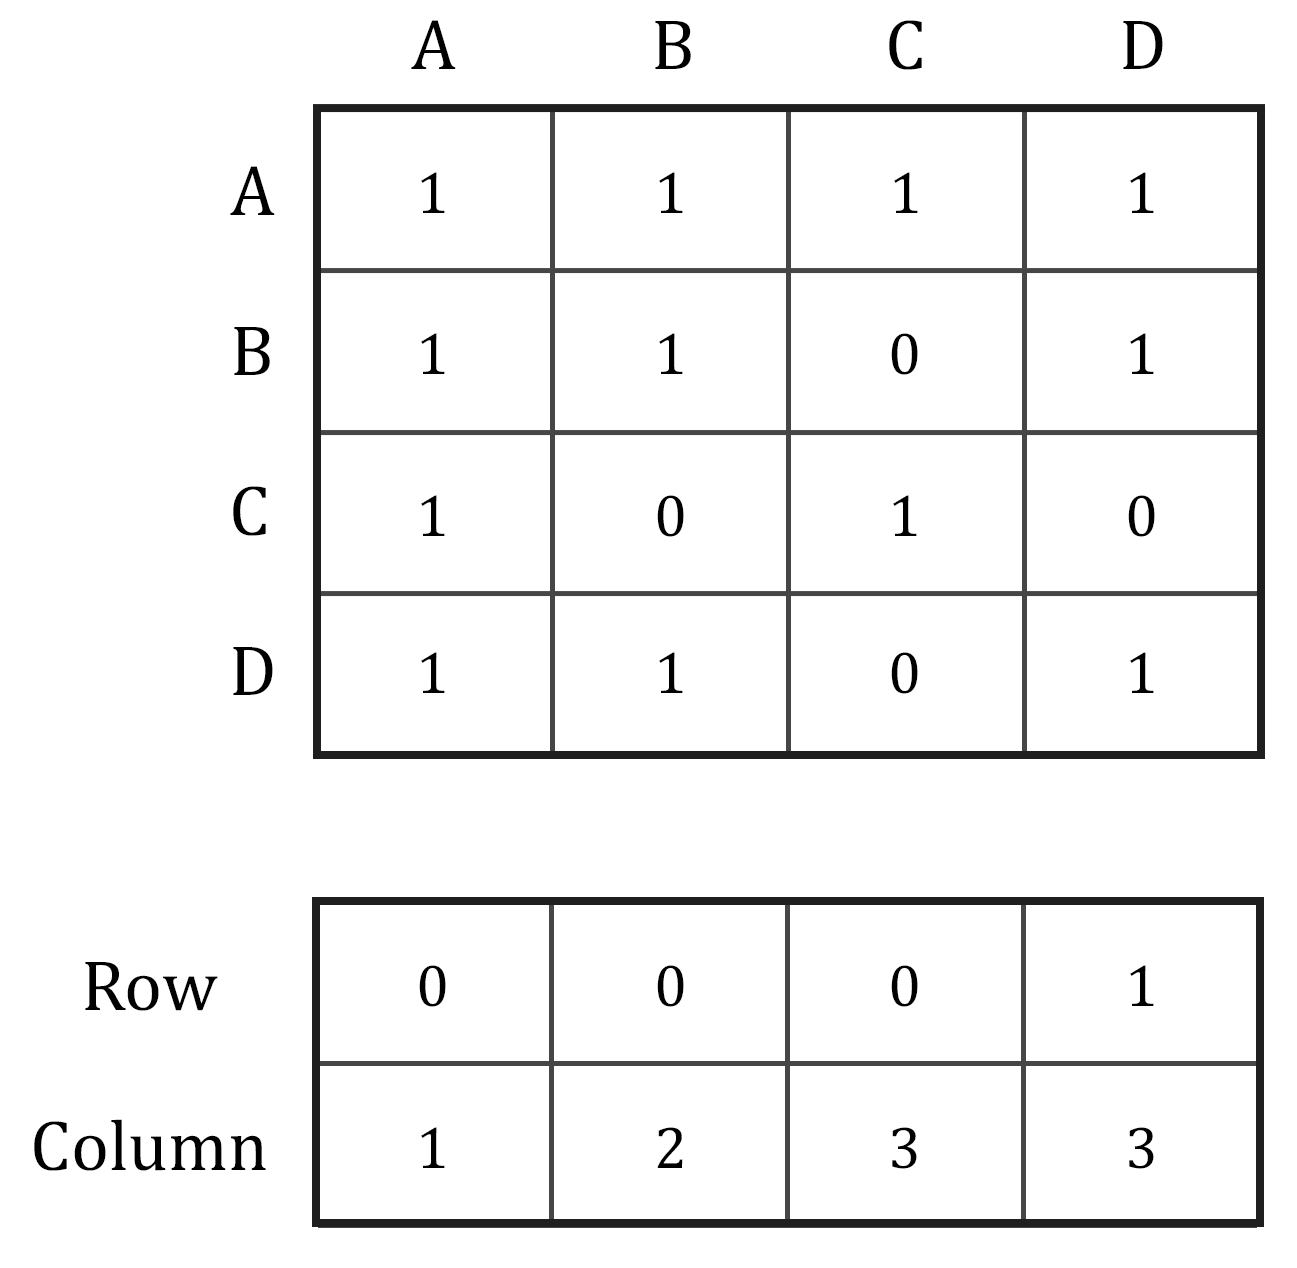
\includegraphics[width=\linewidth]{plots/graph_storing_types.png}
        \captionof{figure}{Adjacency matrix and an edge list for an undirected, unweighted graph}
        \label{fig:graph_storage}
    \end{minipage}
\end{minipage}

\vspace{0.5em}

There are several classifications of graphs that need mentioning (see Figure \ref{fig:graph_types}). The first of them is directed or undirected graphs. It refers to graph edges being one-sided only or always two-sided. An example of an undirected graph could be chemical connections between molecules, and an example of a directed graph could represent task scheduling (task B cannot be done before task A is completed). In a directed graph (or digraph), edges are ordered pairs $(x, y)$, indicating a direction from $x$ to $y$. Thus, in general, $(x, y) \in E$ does not imply $(y, x) \in E$. In contrast, in an undirected graph, edges are unordered pairs, so $\{x, y\} \in E$ is identical to $\{y, x\} \in E$.

Graphs can also be weighted or unweighted. In a weighted graph, each edge $e \in E$ is associated with a weight, which assigns a real-valued value to each edge. In an unweighted graph, all edges are considered to have equal weight.

\vspace{0.5em}

Graphs can be represented in several ways on a computer. Two of the most common representations, and the ones most relevant in this work, are the adjacency matrix and the edge list (see examples for an undirected unweighted graph in Figure \ref{fig:graph_types} on Figure \ref{fig:graph_storage}).

An adjacency matrix for a graph with $n = |V|$ vertices is a matrix $A \in \mathbb{R}^{n \times n}$ where rows and columns correspond to vertices. In the unweighted case, the entries are defined as
\begin{equation}
A_{ij} =
\begin{cases}
1, & \text{if } (v_i, v_j) \in E, \\
0, & \text{otherwise}.
\end{cases}
\end{equation}
For undirected graphs, the adjacency matrix is symmetric, i.e., $A_{ij} = A_{ji}$.

In the weighted case, the entries of the matrix store edge weights instead of binary values, i.e., $A_{ij} = w(v_i, v_j)$ if $(v_i, v_j) \in E$, and $0$ otherwise.

Since the adjacency matrix requires $\mathcal{O}(|V|^2)$ memory, in many modern machine learning frameworks, graphs are commonly represented using an edge index format \cite{fey2019pytorchgeometric}. This consists of a matrix of size $2 \times |E|$, where each column represents an edge by storing the indices of its two endpoints. Additional node features are stored in a matrix $X \in \mathbb{R}^{|V| \times d}$, where $d$ is the number of features per node.


\subsection{Artificial Neural Networks}

Artificial neural networks (ANNs) \cite{goodfellow2016deep} are a class of models inspired by the structure and function of biological neurons in a human brain. Contemporarily, ANNs are used for a wide variety of tasks; however, in this chapter we will focus specifically on their application in supervised learning, since it is the main subject of this work.

Supervised learning refers to a machine learning paradigm in which the model is trained using a dataset containing input samples together with their corresponding correct output labels. During training, the model learns the relationship between the input data and the target labels in order to correctly predict the value of previously unseen samples.

A single artificial neuron (see Figure \ref{fig:single_neuron}) can be simply understood as a linear function with a non-linear activation in the end. It takes $n$ input values $x_1, \dots, x_n \in \mathbb{R}$, each associated with a learnable weight $w_1, \dots, w_n \in \mathbb{R}$. In addition, the neuron has a bias term $b \in \mathbb{R}$ and an activation function $\alpha$.

\begin{minipage}{\textwidth}
    \centering
    \begin{minipage}[t]{0.70\textwidth}
        \centering
        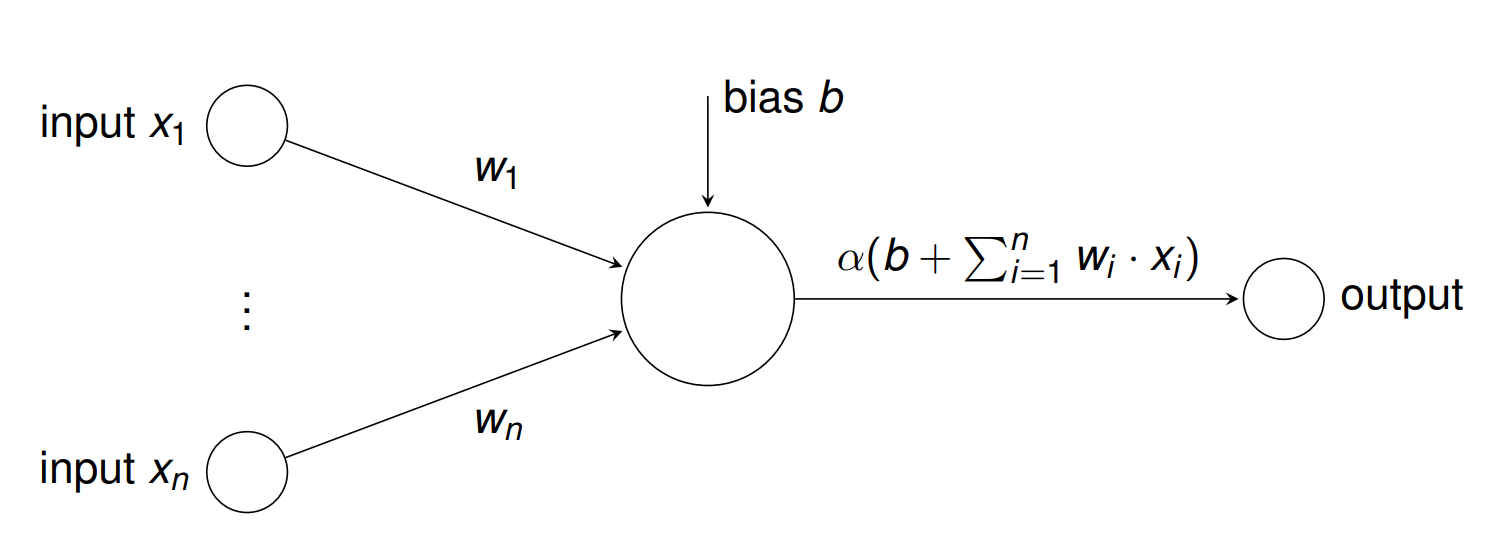
\includegraphics[width=\linewidth]{plots/single_neuron.png}
        \captionof{figure}{A single neuron of an ANN}
        \label{fig:single_neuron}
    \end{minipage}
    \begin{minipage}[t]{0.29\textwidth}
        \centering
        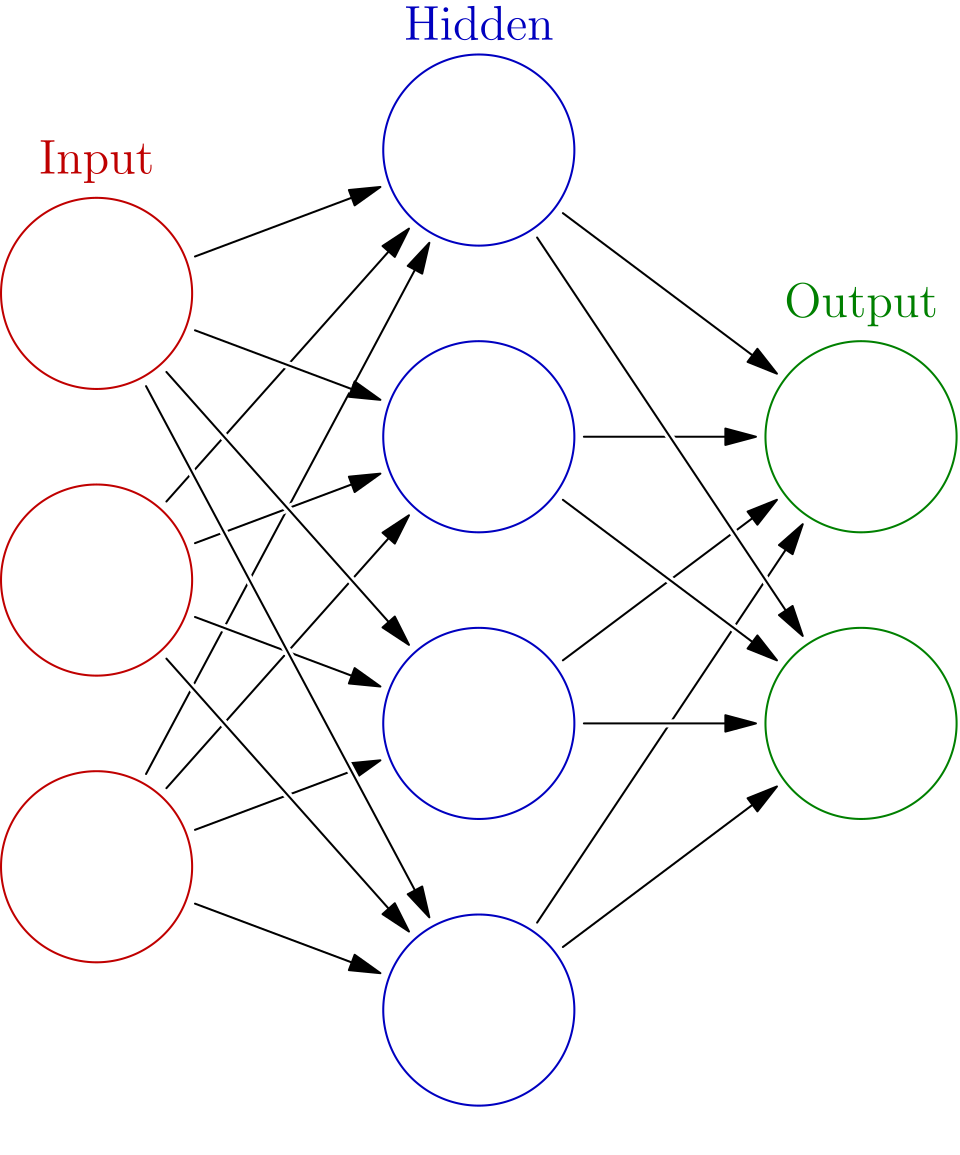
\includegraphics[width=\linewidth]{plots/Colored_neural_network.svg.png}
        \captionof{figure}{An example of a fully connected multilayer perceptron (MLP) with one hidden layer}
        \label{fig:mlp_example}
    \end{minipage}
\end{minipage}

The output of a single neuron is given by
\begin{equation}
\alpha\left( b + \sum_{i=1}^{n} w_i x_i \right).
\end{equation}

The activation function $\alpha$ is a differentiable nonlinear function, which introduces nonlinearity into the model and enables the network to learn complex patterns \cite{goodfellow2016deep}..

Commonly used activation functions include the Rectified Linear Unit \cite{nair2010relu} and the sigmoid function \cite{arai2025intelligent}[p. 481-512], defined as
\begin{equation}
\text{ReLU}(x) = \max(0, x),
\end{equation}
\begin{equation}
\sigma(x) = \frac{1}{1 + e^{-x}}.
\end{equation}

ReLU has become the default choice in many deep learning architectures due to its simplicity, computational efficiency, and favorable gradient propagation properties. The sigmoid function is often used when outputs need to be interpreted as probabilities, as it maps real-valued inputs to the interval [0,1], making it particularly suitable for binary classification tasks.

By stacking multiple neurons into layers, one obtains a multilayer perceptron (MLP), also known as a feedforward neural network. Such networks consist of an input layer, one or more hidden layers, and an output layer (see Figure \ref{fig:mlp_example}). 

MLPs are typically represented as fully connected architectures, meaning that each neuron in a layer is connected to every neuron in the next layer. However, in practice, the effective connectivity can be reduced, for example by learning weights that are close to zero, which diminishes the influence of certain connections.

Given $n$ - the dimentiallity of the input space and $m$ - the dimentiallity of the output space, the training objective in supervised learning is to approximate an unknown function $f_{\theta} : \mathbb{R}^n \rightarrow \mathbb{R}^m$ such that the model fits the given input--output pairs. $\theta$ here represents all the parameters of an ANN such as weights and biases. This is achieved by minimizing a loss function, which measures how well the model's predictions match the true outputs.

There are several loss functions used in practice. For example, given a groung truth $y_i$ of an $i$-th sample of the dataset and the corresponding prediction of a model $\hat y = f_{\theta}(x_i)$, the $0$--$1$ loss is defined as

\begin{equation}
L_{0\text{-}1}(\hat{y_i}, y_i) = \mathbf{1}_{\hat{y_i} \neq y_i},
\end{equation}
which assigns a loss of $1$ when the prediction is incorrect and $0$ otherwise. However, this loss is not differentiable and is therefore not suitable for gradient-based optimization.

A commonly used alternative is the quadratic (or mean squared) loss:
\begin{equation}
L_{\text{quadratic}}(\hat{y_i}, y_i) = (\hat{y_i} - y_i)^2,
\end{equation}
which could be interpreted as an eucliadian distance between the models output and the ground truth.

Given a dataset with $N$ samples, the total loss is typically computed as the average over all samples:
\begin{equation}
\mathcal{L} = \frac{1}{N} \sum_{i=1}^{N} L(\hat{y}_i, y_i),
\end{equation}

giving the formal objective of the neural networks training as

\begin{equation}
\theta^{*} = \arg\min_{\theta} \mathcal{L}\bigl(f_{\theta}(x_i), y_i\bigr)
\end{equation}

This optimization is commonly performed using gradient-based methods such as gradient descent. The key idea is to iteratively update the model parameters in the direction that reduces the loss.

To do this efficiently, neural networks use the backpropagation algorithm. Backpropagation computes the gradient of the loss function with respect to all model parameters by applying the chain rule of calculus.

Consider a neural network with loss function $\mathcal{L}$ and layer activations defined as

\begin{equation}
a^{(l)} = \sigma\left(z^{(l)}\right),
\end{equation}

where

\begin{equation}
z^{(l)} = W^{(l)} a^{(l-1)} + b^{(l)},
\end{equation}

with $W^{(l)}$ denoting the weight matrix, $b^{(l)}$ the bias vector, $\sigma(\cdot)$ the activation function, and $a^{(l-1)}$ the output of the previous layer. Then the derivitive of the loss function by the weights and applied the chain rule is given by

\begin{equation}
\frac{\partial \mathcal{L}}{\partial W^{(l)}} =
\frac{\partial \mathcal{L}}{\partial a^{(l)}}
\frac{\partial a^{(l)}}{\partial z^{(l)}}
\frac{\partial z^{(l)}}{\partial W^{(l)}}.
\end{equation}

Then the error term for layer $l$ can be defined as

\begin{equation}
\delta^{(l)} =
\frac{\partial \mathcal{L}}{\partial z^{(l)}},
\end{equation}

which can be propagated backward through the network according to

\begin{equation}
\delta^{(l)} =
\left( W^{(l+1)T} \delta^{(l+1)} \right)
\odot \sigma'\left(z^{(l)}\right),
\end{equation}

where $\odot$ denotes element-wise multiplication and $\sigma'(\cdot)$ is the derivative of the activation function.

Using the computed gradients, the network parameters are updated through gradient-based optimization methods such as gradient descent:

\begin{equation}
W^{(l)} \leftarrow
W^{(l)} - \eta
\frac{\partial \mathcal{L}}{\partial W^{(l)}},
\end{equation}

where $\eta$ represents the learning rate.

Training is can also be performed iteratively over the dataset in mini-batches of size $B$. Instead of updating the parameters after processing the entire dataset, the gradients are computed for each mini-batch and used to perform intermediate parameter updates. One complete pass over all training samples is referred to as an epoch. The training procedure is repeated for a predefined number of epochs until the model converges or the optimization process is terminated.

By repeatedly applying forward propagation, loss computation, backpropagation, and parameter updates over multiple mini-batches and epochs, the network gradually improves its performance and converges to a set of parameters that (locally) minimize the loss.

Having said that, the choice of the learning rate can be crucial to the process. By choosing a learning rate that is too high or too low, the loss may decrease too slowly or even increase. The intuition for this effect is shown in Figure \ref{fig:learning_rate}.


\begin{minipage}{\textwidth}
    \centering
    \begin{minipage}[t]{0.65\textwidth}
        \centering
        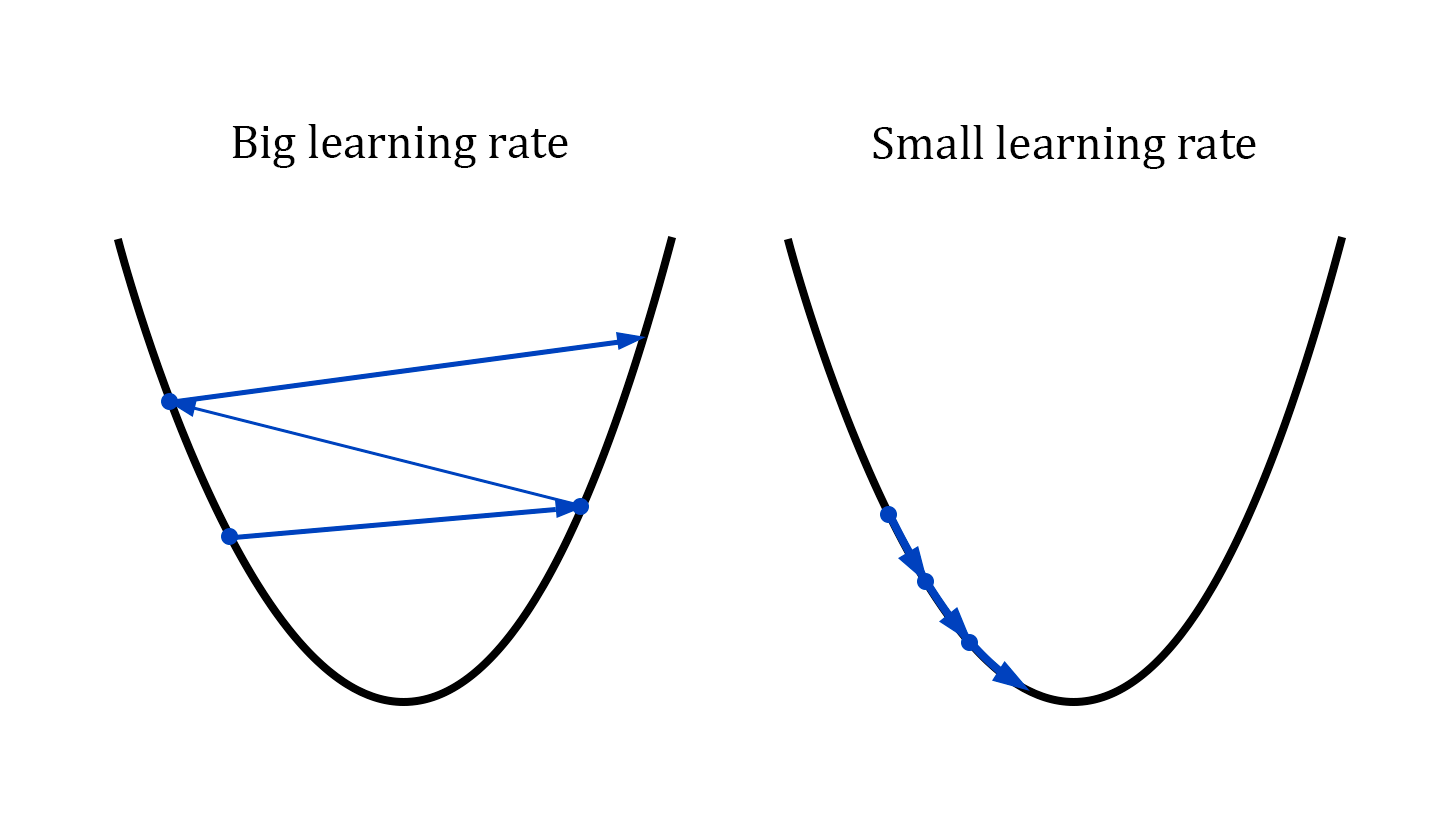
\includegraphics[width=\linewidth]{plots/learning_rate.png}
        \captionof{figure}{Illustration of the importance of the learning rate}
        \label{fig:learning_rate}
    \end{minipage}
\end{minipage}


\subsection{Anomaly Detection with Graph Neural Networks}

Anomaly detection is a field that focuses on identifying unusual or unexpected patterns in data. Such patterns are also referred to as anomalies. With the increasing use of graph-structured data \cite{wu2021gnnsurvey}, it has become important to develop methods for detecting anomalies in graphs as well. In this section, we present Graph Isomorphism Networks, which are widely used for anomaly detection tasks in graph data \cite{xu2019gin}.

Graph anomaly detection problems can vary significantly depending on their objective. A model is typically trained for a specific task, which can be categorized into different levels of graph anomaly detection. The most common levels are graph-level, node-level, edge-level, and subgraph-level anomaly detection. Each of these levels defines what is considered an anomaly in a different way.

In graph-level anomaly detection, the goal is to determine whether an entire graph is anomalous. In node-level anomaly detection, the objective is to identify anomalous nodes within a graph. Similarly, edge-level anomaly detection focuses on detecting unusual connections, while subgraph-level anomaly detection aims to identify anomalous patterns or structures within subsets of the graph. 

Going further, we will consider only node- and graph-level anomaly tasks, since these are the ones which are relevant for this work.

\subsubsection{Graph Isomorphism Networks}

Neural networks that operate on graph data and learn embeddings (mappings of complex high-dimentional data into a lower-dimensional vector space) for nodes are called graph neural networks (GNNs). Their mechanism is based on exchanging information between neighbors and updating node attributes, which is particularly effective due to the clustering properties commonly observed in real-world graphs. Graph Isomorphism Networks (GIN) are GNNs which aggregate information between neighbors (also called message passing) by a sum, which was proven to have the most expressive power \cite{xu2019gin}, and an MLP to learn complex patterns.

\vspace{0.5em}

\begin{minipage}{\textwidth}
    \centering
    \begin{minipage}[t]{0.75\textwidth}
        \centering
        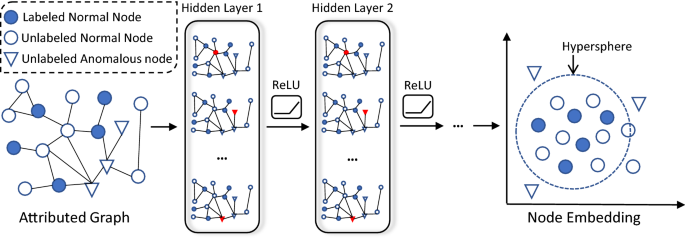
\includegraphics[width=\linewidth]{plots/ocgin.png}
        \captionof{figure}{Structure of an OCGIN model \cite{ocgin}}
        \label{fig:ocgin}
    \end{minipage}
\end{minipage}

\vspace{0.5em}

Given a graph $G = (V, E)$, a node attribute matrix $X \in R^{n \times m}$, where $n$ is the number of nodes and $m$ is the dimensionality of the feature vector, is initialized as:

\begin{equation}
h^0_i = x_i \forall i=1..n
\end{equation}

For layer $k$ and node $i$, the update step is given by:

\begin{equation}
h_i^{(k)} = \mathrm{MLP}^{(k)} ( h_i^{(k-1)} + \alpha \cdot \sum_{ j \in N(i) } h^{k-1}_j), 
\end{equation}

which is also referred to as a GIN layer. Since message passing (mehrere MLPs erwähnen / kontretisieren) is performed at every layer, the receptive field of each node grows with depth. To be exact, after $k$ layers, the representation $h_i^{(k)}$ contains information from nodes up to $k$ steps away from the original node.

To obtain a single representation for a graph or a node, pooling operations are applied to node embeddings. Common pooling methods include mean, max, and min pooling. Given node embeddings $\{h_i^{(k)}\}_{i \in V(G)}$ across $L$ layers, a simple mean pooling for graph-level AD is defined as

\begin{equation}
h_G = \frac{1}{|V(G)| \cdot L} \sum_{k=1}^{L} \sum_{i \in V(G)} h_i^{(k)}.
\end{equation}

In contrast, for node-level anomaly detection, the final pooling step is omitted. Instead, the model produces an embedding $h_i$ for each node, allowing anomaly scores to be computed individually per node.

\begin{equation}
h_i = \frac{1}{L} \sum_{k=1}^{L} h_i^{(k)}.
\end{equation}

In order to make such aggregation possible, the input and output dimensionalities of the layers of the MLPs have to be consistent, aside from the first input layer.

Since this approach used for anomaly detection in this setting is based on hypersphere learning, inspired by methods such as SVDD \cite{pmlr-v80-ruff18a}, the idea is to map the computed normal embeddings $h_i$ or $h_G$ close to a center $c \in \mathbb{R}^d$ in the embedding space, while anomalies are expected to lie further away. The formal objective can be given by:

\begin{equation}
\min_{\theta} \sum_{i} 
\left\| f_\theta(G_i) - c \right\|^2.
\end{equation}

In practice, it is typically pre-computed with the initialized random weights.

The loss function of an OCGIN is therefore the squared distance between the embedding and the center:
\begin{equation}
\mathcal{L} = \frac{1}{N} \sum_{i=1}^{N} \| h_i - c \|^2.
\end{equation}

The objective of the model is to minimize this loss, thereby pulling normal data points closer to the center of the hypersphere. However, this formulation introduces a potential issue: the model may converge to a trivial solution in which all embeddings collapse to the center, effectively shrinking the hypersphere to a single point \cite{pmlr-v80-ruff18a}. This phenomenon is called hypersphere collapse.

Such behavior is a known challenge in one-class graph anomaly detection models like OCGIN. To mitigate this, additional constraints or regularization techniques are often employed. For example, approaches such as OCGTL construct ensembles of models (e.g., using generative adversarial networks) with different objectives to improve robustness and avoid trivial solutions \cite{wang2024ocgtl}.

\subsubsection{Classification using a trained OCGIN model}

Predictions in an OCGIN are based on anomaly scores, which measure how far a given entity (e.g., a node or a graph) is from the center of a hypersphere. For example, for node- or graph-level embeddings $h_i$, the anomaly score can be defined as
\begin{equation}
a_i = \| h_i - c \|^2,
\end{equation}
where $c$ is the center of the hypersphere.

However, many evaluation metrics require binary predictions rather than continuous scores. Therefore, anomaly scores must be converted into labels. Two common approaches are used for this purpose.

The first approach is to determine a threshold based on the training data. For example, one may choose a threshold corresponding to a high quantile (e.g., $95\%$) of the training anomaly scores. Any sample with a score above this threshold is classified as anomalous. % A drawback of this method is that it assumes all training data is normal, which may lead to underestimation if anomalies are present in the training set.

The second approach introduces a validation set (resulting in a train/validation/test split). Since the validation set contains labeled normal and anomalous samples, it can be used to select an optimal threshold. For example, the threshold can be chosen to maximize a performance metric such as accuracy or minimize an impurity measure such as the Gini index (discussed in section \ref{sec:methodology}).

The threshold in this work is selected using Youden’s J statistic \cite{youden1950index} (also referred to as Youden’s index), which provides a criterion for balancing the trade-off between true positive and false positive rates. The metric is commonly used in binary classification and anomaly detection to identify the operating point that maximizes the separation between normal and anomalous samples. Formally, Youden’s J statistic is defined as the sum of sensitivity (true positive rate) and specificity (true negative rate) (see Chapter \ref{eval}) minus one:

\begin{equation}
J = \text{Sensitivity} + \text{Specificity} - 1
\end{equation}

A higher value of \(J\) indicates better discriminatory performance, with the maximum possible value of \(1\) corresponding to perfect classification. During validation, the anomaly score threshold is varied across possible values, and the threshold yielding the highest Youden’s J statistic is selected. This approach ensures that both the detection of anomalies and the correct classification of normal samples are considered simultaneously, making it particularly suitable for anomaly detection settings with imbalanced class distributions.

Once the threshold is determined, it defines a decision boundary: samples with scores below the threshold are considered normal, while those above it are classified as anomalous. The model can then be evaluated on the test set.

% TODO ist halt scheisse, dass hier zuerst validation set und erst dann die motivation fuers splitten ist

\subsection{Evaluation of Graph Anomaly Detection Models}

The evaluation of any artificial neural network is based on the idea that a model cannot be evaluated on the same data on which it was trained, since it would make the analysis sensitive to overfitting \cite{goodfellow2016deep}. The solution to this is splitting the dataset into at least two parts: a training set and a test set. The model is trained on the training data and then evaluated on the test data by comparing its predictions with the true labels.

A particular challenge in anomaly detection is, in many cases, the training data consists only of normal samples. Such datasets, where one class is represented more then the pthers are called imbalanced. As a result, special care must be taken when constructing evaluation datasets. In practice, evaluation often requires labeled data containing both normal and anomalous examples. Other than that, most evaluation techniques for binary classification can be used here too.

\subsubsection{Evaluation Methods for Binary Classification}
\label{eval}

The evaluation of binary classification can be formulated as follows: given true labels $y \in \{0,1\}^n$ and predicted labels $\hat{y} \in \{0,1\}^n$, we aim to measure how well the model performs.

A simple evaluation metric is the accuracy (or test rate), defined as
\begin{equation}
\text{accuracy} = \frac{1}{n} \sum_{i=1}^{n} \mathbf{1}_{\hat{y}_i = y_i}.
\end{equation}
This metric measures the proportion of correctly classified samples over the total.

However, accuracy can be misleading when the dataset is imbalanced. To better understand model performance, it is useful to consider the confusion matrix, which summarizes the possible prediction outcomes:

\begin{itemize}
    \item True Positive (TP): correctly predicted anomalies,
    \item True Negative (TN): correctly predicted normal samples,
    \item False Positive (FP): normal samples incorrectly classified as anomalies,
    \item False Negative (FN): anomalies incorrectly classified as normal.
\end{itemize}

\begin{minipage}{\textwidth}
    \centering
    \begin{minipage}[t]{0.65\textwidth}
        \centering
        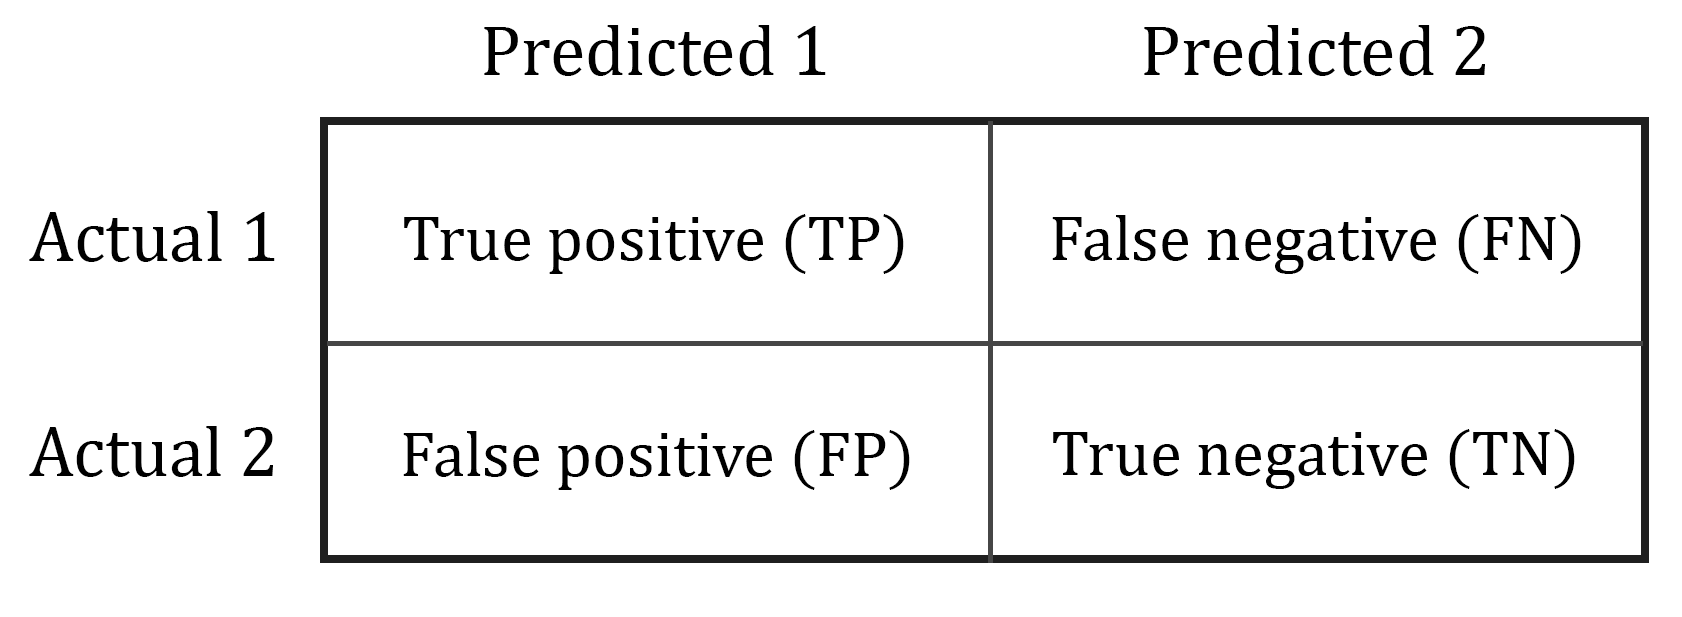
\includegraphics[width=\linewidth]{plots/confusion_matrix.png}
        \captionof{figure}{Confusion matrix}
        \label{fig:confusion_matrix}
    \end{minipage}
\end{minipage}

Based on these quantities, several important evaluation metrics can be defined. Precision and recall are given by
\begin{equation}
\text{precision} = \frac{TP}{TP + FP}, \qquad
\text{recall} = \frac{TP}{TP + FN}.
\end{equation}

Precision measures how many predicted anomalies are actually anomalous, while recall measures how many of the true anomalies were correctly detected.

Taking a mean out of precision and recall we receive another metric, called balanced accuracy. It is designed to handle imbalanced datasets, since it is not biased by possibly unequal number of positive and negative labels. Balanced accuracy is given by: 

\begin{equation}
\text{balanced accuracy} = \frac{1}{2} \left( \frac{TP}{TP + FN} + \frac{TN}{TN + FP} \right).
\end{equation}

F1 Score uses precision and recall just like balanced accuracy, but uses multiplication of two devided by the sum, which punishes inbalance between two more: 

\begin{equation}
F_1 = 2 \cdot \frac{\text{precision} \cdot \text{recall}}{\text{precision} + \text{recall}}.
\end{equation}

Another important metric is the Area Under the Receiver Operating Characteristic Curve (AUC-ROC). The ROC curve plots the true positive rate (recall) against the false positive rate, given a threshold $t$. The idea is that most binary classifiers do not output a direct binary prediction, but rather a real number between 0 and 1, so the choice of the threshold is vital to the predictive power of the model.

Given true labels $y \in \{0,1\}^n$ and predicted continuous values $\hat{y} \in [0,1]^n$ and a real value $t \in [0, 1]$, compute

\begin{equation}
    p_i^t = 1_{\hat y_i > t}, \qquad
    TP(t) = \sum_{i}1_{y_i = 1, p_i^t = 1}, \qquad
    FP(t) = \sum_{i}1_{y_i = 0, p_i^t = 1}.
\end{equation}

and the true positive rate and false positive rate as:

\begin{equation}
\text{TPR}(t) = \frac{TP(t)}{TP(t) + FN(t)}, \qquad
\text{FPR}(t) = \frac{FP(t)}{FP(t) + TN(t)}.
\end{equation}

$TPR(t)$ and $FPR(t)$ can be plotted on an x-y axis. The intuition for this is as follows: the bigger the $t$ value is, the more samples are classified as zero, and the bigger the false negative rate should get, and vice versa. But the more "sure" the model is of its predictions (if the true label is one, the output of a model $\to 1$), the less the false positive rate will be, even with increasing $t$. This means that, with random guessing, the values $p^t$ will be randomly scattered across the $[0, 1]$ region, so the ROC-AUC curve will look like a linear $y=x$ function. The better the model gets at guessing, and the more sure the model is of the guess, the more the curve will concentrate at the upper left corner of the ROC-AUC curve (see Figure \ref{fig:roc_auc}).

\begin{minipage}{\textwidth}
    \centering
    \begin{minipage}[t]{0.65\textwidth}
        \centering
        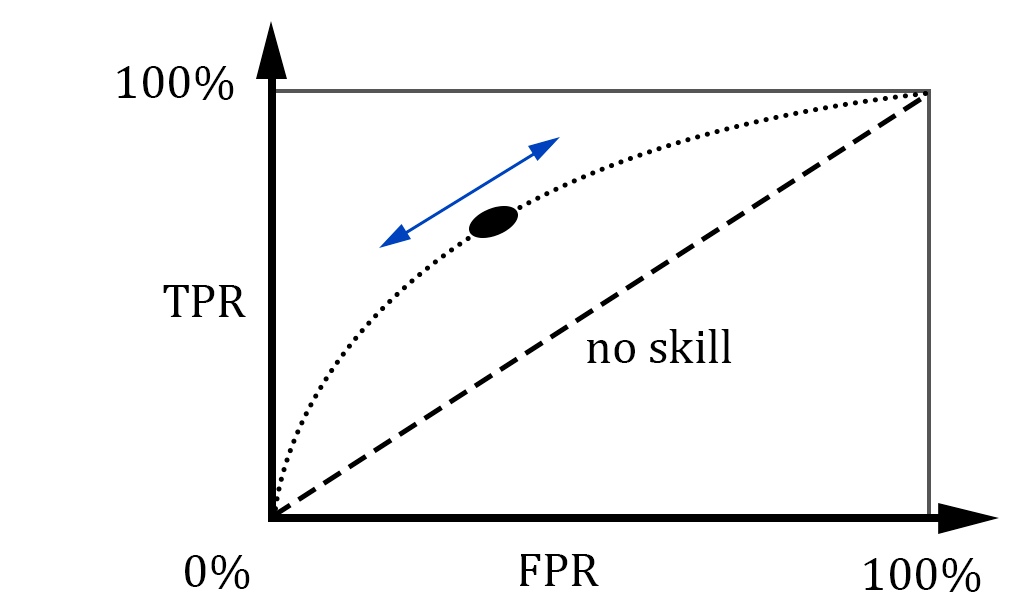
\includegraphics[width=\linewidth]{plots/roc_auc.png}
        \captionof{figure}{Examples of ROC-AUC curves}
        \label{fig:roc_auc}
    \end{minipage}
\end{minipage}

The Area Under the ROC Curve can be integrated, and it can be interpreted as the probability that the model ranks a randomly chosen anomalous sample higher than a randomly chosen normal sample. A value of $0.5$ corresponds to random guessing, while a value of $1$ indicates perfect separation.

The ROC-AUC value is central to the evaluation of binary classification models, since it does not depend on a fixed classification threshold and is not biased by the imbalance of the dataset.

\subsection{Logical Constrains in Deep Learning}

Logical constraints are a field in deep learning that has attracted especially high interest in recent years. Papers \cite{Giunchiglia_2022}, \cite{stoian2024realisticsyntheticdataconstraining} on the topic show that, by implementing logical rules in the learning process, one can improve performance, learn from less data, and improve interpretability. A major source of motivation is that most neural networks in practice are either domain-agnostic or have to obey certain rules. These could be, for example, physical laws.

Logical constraints are formal rules that restrict the behavior of a machine learning model according to predefined relationships or domain knowledge. In deep learning, these constraints are used to ensure that the predictions of a neural network satisfy certain logical conditions in addition to fitting the training data.

Logical constraints in deep learning are generally categorized into two types: hard and soft constraints.

Hard constraints \cite{kotary2021constrained} must never be violated. They represent strict requirements that the model output has to satisfy under all circumstances. Hard constraints are commonly enforced through constrained optimization or symbolic reasoning methods.

Soft constraints \cite{Giunchiglia_2022} allow occasional violations but introduce penalties when constraints are not satisfied. Instead of enforcing absolute correctness, they encourage the model to prefer logically consistent solutions. Soft constraints are particularly important in modern deep learning because they can be integrated into differentiable optimization procedures.

In this section we will first look into mostly used logical formalisms, then we discuss methods of differentiable logic and in the end we will present some modern approaches of introducing logic into deep learning models.

\subsubsection{Logical Formalisms}

Logical formalizations provide a precise mathematical language for representing and reasoning about constraints, relations, and inference.  Several logical formalisms are commonly used in machine learning, such as propositional logic or first-order logic \cite{endelerton2001logic}. In this subsection we briefly discuss the most used ones.

\paragraph{Propositional Logic.}

Propositional logic is based on atomic propositions $p_1, p_2, \dots, p_n$ which evaluate to either \emph{true} or \emph{false}. Complex formulas are constructed using logical connectives such as conjunction \((\land)\), disjunction \((\lor)\), negation \((\neg)\), implication \((\rightarrow)\), and equivalence \((\leftrightarrow)\).

A propositional formula is interpreted under a valuation
\begin{equation}
\nu : \{p_1,\dots,p_n\} \rightarrow \{\top,\bot\},
\end{equation}
which assigns a truth value to each proposition. A formula is satisfiable if there exists a valuation under which the formula evaluates to true.

\paragraph{First-Order Logic.}
First-order logic (FOL) extends propositional logic by introducing variables, predicates, functions, and quantifiers. Let $x_1, x_2, \dots x_N $ denote variables over a domain \(D\). Predicates express relations over elements of \(D\), while function symbols represent mappings within the domain and quantifiers limit the domain space, to which the logic is applied.

Formulas in first-order logic are constructed using the universal quantifier $\forall$ and the existential quantifier $\exists$. For example,
\begin{equation}
\forall x \, (P(x) \rightarrow Q(x))
\end{equation}
states that every element satisfying \(P\) also satisfies \(Q\)

Though satisfiability in first-order logic is undecidable \cite{endelerton2001logic}, compared to propositional logic, first-order logic is significantly more expressive and allows formalization of relational constraints. 

\subsubsection{Differentiable Logic}

A major challenge in combining logic with neural networks is that classical Boolean logic is not differentiable. Neural networks, however, rely on gradient-based optimization methods that require differentiable operations. Differentiable logic addresses this issue by replacing discrete truth values with continuous truth degrees in the interval $[0,1]$, where \(0\) denotes complete falsity and \(1\) complete tautology.

A common foundation for differentiable logic is given by fuzzy logics and continuous \(t\)-norm semantics. Let
\begin{equation}
a,b \in [0,1]
\end{equation}
denote continuous truth values. A \(t\)-norm
\begin{equation}
T(a,b)
\end{equation}
generalizes logical conjunction, while corresponding \(t\)-conorms generalize disjunction. Different choices of these operators lead to different logical systems with distinct semantic properties.

Fuzzy logic generalizes Boolean logic by allowing partial truth values in the interval \([0,1]\). Instead of strict binary evaluation, propositions may hold to a certain degree. This framework is particularly suitable for differentiable reasoning because logical operators can be represented by continuous or piecewise differentiable functions. Important distunquish between differentiable logic and fuzzy logic: fuzzy logic systems are not always differentiable, and were designed to handle uncertanty, while differentiable Logic uses differentiable parts of fuzzy logic in order to construct a framework used in Deep learning. In following we will discusses most known fuzzy logic systems.

\paragraph{Łukasiewicz Logic.}
Łukasiewicz logic defines conjunction and disjunction using bounded linear operators. The conjunction operator is given by
\begin{equation}
a \land b = \max(0, a+b-1),
\end{equation}
while disjunction is defined as
\begin{equation}
a \lor b = \min(1, a+b).
\end{equation}
Negation is expressed as
\begin{equation}
\neg a = 1-a.
\end{equation}
Łukasiewicz logic is attractive in differentiable systems because its operators are continuous and piecewise linear, leading to stable gradients during optimization.

\paragraph{Gödel Logic.}
Gödel logic defines conjunction and disjunction through minimum and maximum operators:
\begin{equation}
a \land b = \min(a,b),
\qquad
a \lor b = \max(a,b).
\end{equation}
Negation is commonly defined as
\begin{equation}
\neg a =
\begin{cases}
1 & \text{if } a=0, \\
0 & \text{otherwise}.
\end{cases}
\end{equation}
Gödel logic preserves an ordering-based interpretation of truth and is closely related to intuitionistic and modal logical systems. 

\paragraph{Product Logic.}
Product logic models conjunction using multiplication:
\begin{equation}
a \land b = a \cdot b.
\end{equation}
The corresponding disjunction operator is
\begin{equation}
a \lor b = a + b - a b,
\end{equation}
and negation is typically defined as
\begin{equation}
\neg a =
\begin{cases}
1 & \text{if } a=0, \\
0 & \text{otherwise}.
\end{cases}
\end{equation}
Product logic has a probabilistic interpretation and is particularly suitable when truth values are interpreted as independent probabilities. Due to its smooth multiplicative structure, it is widely used in differentiable reasoning frameworks and probabilistic neural-symbolic systems.

\begin{table}[h]
\centering
\begin{tabular}{l|c|c|c}
\textbf{Logic} & \textbf{Conjunction } (\(\land\)) & \textbf{Disjunction } (\(\lor\)) & \textbf{Negation } (\(\neg\)) \\
\hline
Łukasiewicz &
\(\max(0,a+b-1)\) &
\(\min(1,a+b)\) &
\(1-a\)
\\
Gödel &
\(\min(a,b)\) &
\(\max(a,b)\) &
\(
\begin{cases}
1 & a=0 \\
0 & \text{otherwise}
\end{cases}
\)
\\
Product &
\(a \cdot b\) &
\(a+b-ab\) &
\(
\begin{cases}
1 & a=0 \\
0 & \text{otherwise}
\end{cases}
\)
\\
\end{tabular}
\caption{Differentiable implementations of logical operators in common fuzzy logics.}
\label{tab:differentiable_logics}
\end{table}


\paragraph{Probabilistic Logics.}

Probabilistic logics extend classical logical systems by integrating uncertainty. Instead of assigning formulas only the truth values \(\top\) or \(\bot\), probabilistic approaches associate logical statements with probability distributions or weighted constraints.

A prominent framework is given by Markov Logic Networks (MLNs), which combine first-order logic with Markov networks. Formally, an MLN is defined as a set
\begin{equation}
L = \{(F_1,w_1), \dots, (F_n,w_n)\},
\end{equation}
where each \(F_i\) is a first-order formula and \(w_i \in \mathbb{R}\) is a weight representing the strength of the corresponding constraint. Given a finite set of constants, the formulas induce a grounded Markov network over possible worlds \(x\). The probability distribution over worlds is defined by
\begin{equation}
P(X=x)
=
\frac{1}{Z}
\exp\left(
\sum_i w_i n_i(x)
\right),
\end{equation}
where \(n_i(x)\) denotes the number of satisfied groundings of formula \(F_i\) in the world \(x\), and \(Z\) is the normalization constant (partition function). In contrast to classical logic, formulas in MLNs act as soft constraints: violations reduce probability rather than causing inconsistency.

\subsubsection{Integration of logical rules into deep Learning}

\paragraph{Constraint-Based Loss Functions}

One of the most widely used \cite{xu2018semanticloss} approaches integrates soft logical constraints directly into the training objective through additional loss terms. The key idea is to guide the neural network toward solutions that not only minimize the prediction error but also satisfy domain-specific rules.

The general formulation is:

\begin{equation}
L_{\text{total}} = L_{\text{task}} + \lambda L_{\text{logic}}
\end{equation}

Where:

\begin{itemize}
    \item $L_{\text{task}}$ is the original model loss,
    \item $L_{\text{logic}}$ penalizes logical inconsistencies (e.g. fuzzy logic term),
    \item $\lambda$ determines the importance of the logical constraints.
\end{itemize}

Advantages of this approach include: Easy integration into existing architectures, compatibility with gradient-based optimization and good scalability for large neural networks.

\paragraph{Differentiable Logic Layers.}

An alternative approach embeds logical reasoning directly into the architecture of neural networks through differentiable logic layers \cite{yang2023injectinglogicalconstraintsneural}. Instead of applying logic only as an external regulator, logical operators become trainable computational components within the forward pass of the model. In such architectures, neurons or dedicated modules implement differentiable logical operations such as fuzzy conjunctions, disjunctions, and implications.

Formally, given continuous truth values
\begin{equation}
a_1, \dots, a_n \in [0,1],
\end{equation}
a differentiable logic layer computes
\begin{equation}
y = T(a_1,\dots,a_n),
\end{equation}
where \(T\) is a differentiable relaxation of a logical connective, for example a \(t\)-norm. These layers can be stacked hierarchically to construct complex logical expressions within deep architectures. In contrast to purely symbolic systems (TODO, who), differentiable logic layers allow logical structure and neural representations to be learned jointly through gradient descent.


\subsection{Decision Trees}

In this subsection, we introduce a non-parametric supervised learning method that will be used in later chapters to approximate and learn logical rules from data. While decision trees are among the simplest machine learning models, they are highly interpretable, which makes them widely used in practice.

A decision tree is a tree where nodes represent simple decision rules. Each path from the root to a leaf node defines a conjunction of logical conditions (example: Figure \ref{fig:decision_tree}). These rules are typically based on thresholding individual features. A tree is built by recursively iterating over all possible thresholds for every node and finding the best partition.

\begin{minipage}{\textwidth}
    \centering
    \begin{minipage}[t]{0.65\textwidth}
        \centering
        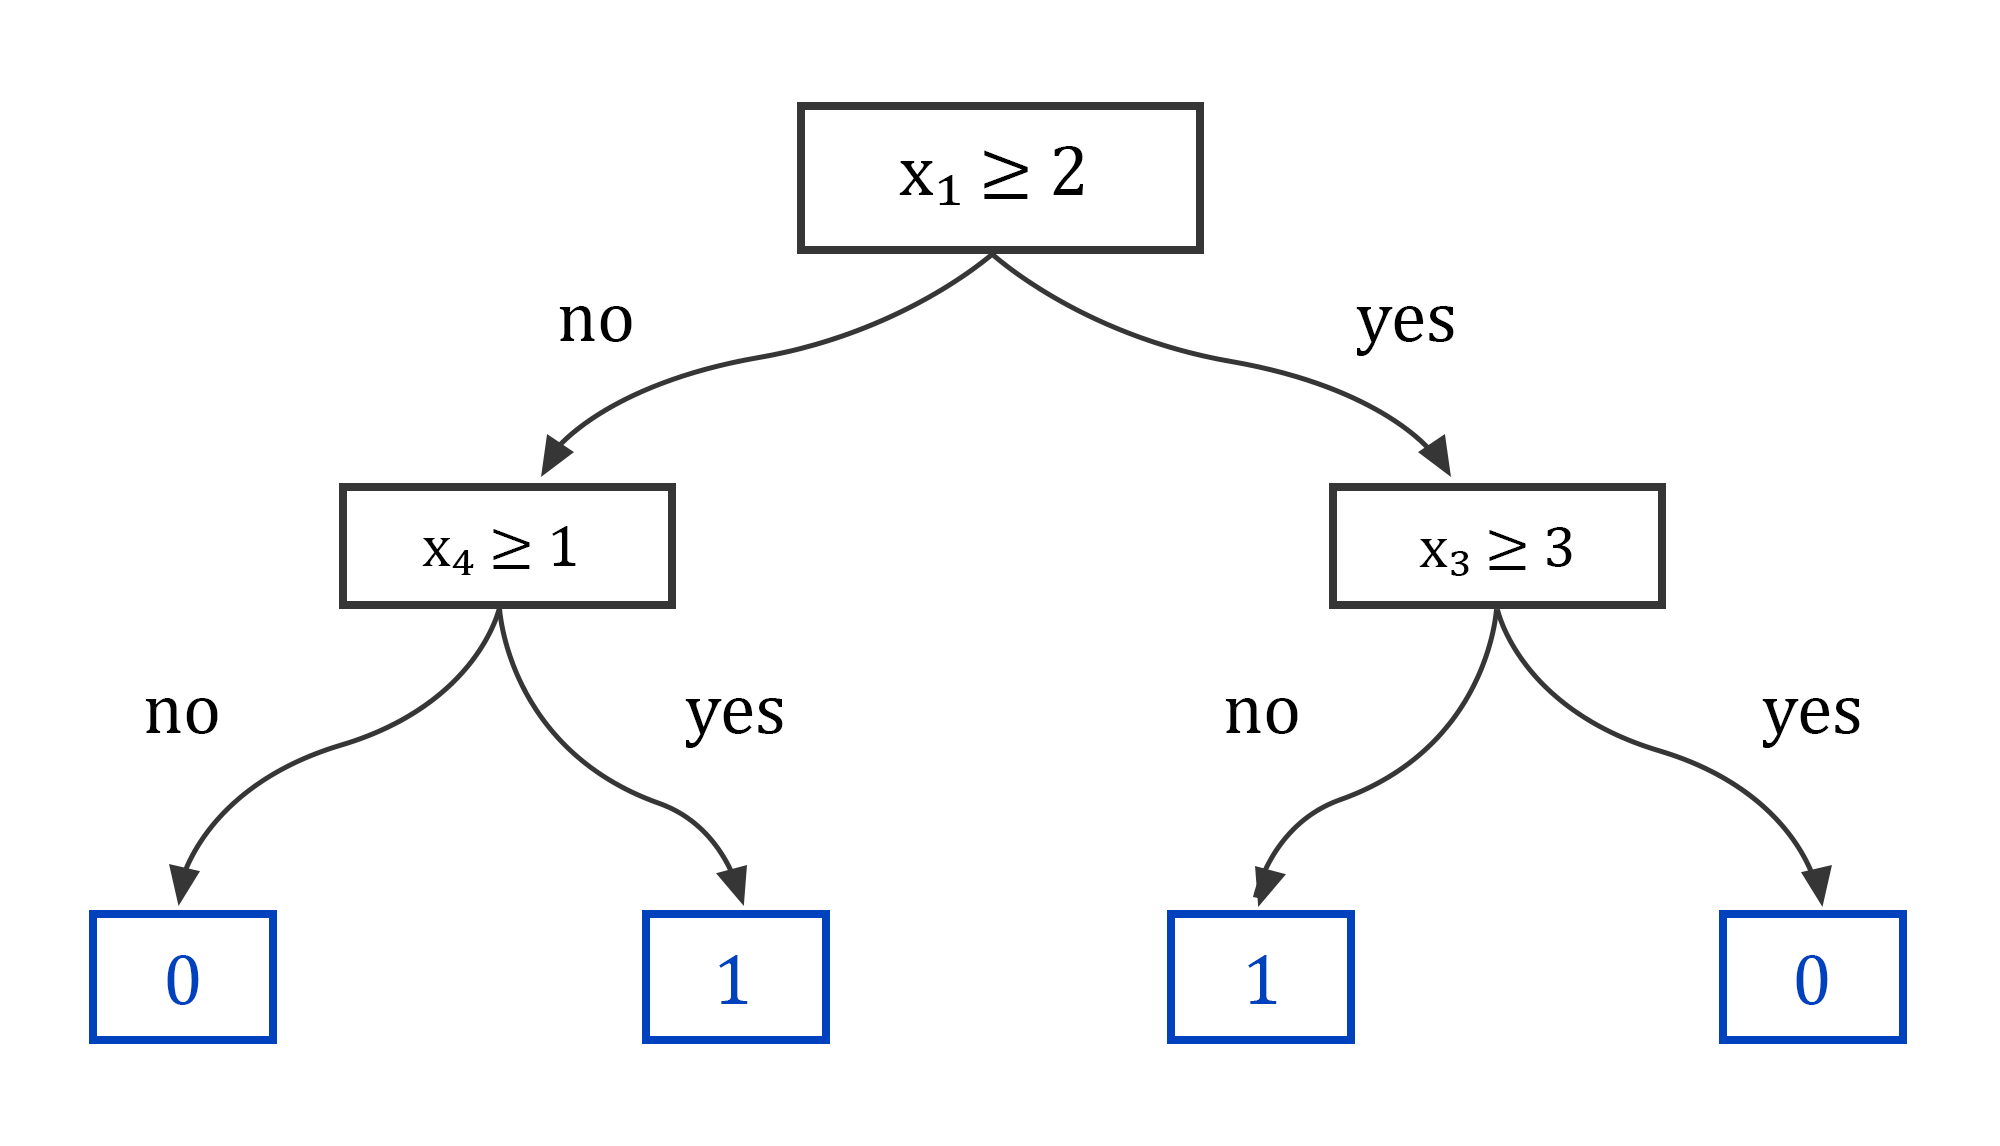
\includegraphics[width=\linewidth]{plots/what-is-a-decision-tree.png}
        \captionof{figure}{An example of a learned decision tree.}
        \label{fig:decision_tree}
    \end{minipage}

\end{minipage}

Formally, let the input space be $\mathcal{X} = \mathbb{R}^d$ and the output space be $\mathcal{Y}$ (e.g., $\mathcal{Y} = \{0,1\}$ for binary classification). A decision tree represents a function $h : \mathcal{X} \rightarrow \mathcal{Y}$.

The hypothesis space of decision trees consists of axis-aligned partitions of the input space. Each internal node of the tree corresponds to a decision rule of the form
\begin{equation}
x_j \leq t,
\end{equation}
where $j \in \{1, \dots, d\}$ is a feature index and $t \in \mathbb{R}$ is a threshold.

Given $S \in \mathcal{X}$, the subset of data for a node, a learning problem is given by:
% TODO f who?

\begin{equation}
    \arg \min_{t \in \mathbb{R}, f\in 1..d} \sum_{K \in \{L, R\}} \frac{|S_K(f, t)|}{|S|} I(S_K(f, t))
\end{equation}

where $S_L$ and $S_R$ are the subsets of $y$ and $X$ less than and greater than the chosen threshold.

\begin{equation}
    S_L = \{x_i,y_i \mid x_{i,f} < t, i\in 1..N\},
\end{equation}

\begin{equation}
    S_R = \{x_i,y_i \mid x_{i,f} \geq t, i\in 1..N\},
\end{equation}

and $I(S_k)$ is an impurity function, which tells how good the selection is. The most common function is the Gini impurity, given by:

\begin{equation}
    I_{\text{gini}}(p) = 1 - \sum_{c \in C}p_c^2
\end{equation}

where $C$ is the set of all classes (in the case of binary classification, it is $\{0, 1\}$) and $p_c$ is the proportion of class $c$ in the set $S_k$.

The tree is constructed in a top-down, greedy manner by recursively splitting the data. At each step, the algorithm selects the feature and threshold that best separate the data according to a chosen criterion.

The algorithm stops either when a given maximum tree depth is achieved or all leaves are pure ($I(S_k) = 0$). Since trees quite often overfit without a stopping criterion, techniques such as pruning can be used to cut off the lower parts of the tree.


\subsection{Differentiable Logic Gate Networks}
\label{sec:dlgt}

Differentiable Logic Gate Networks (DLGNs)~\cite{petersen2022difflogic} are a class of models that learn Boolean circuit structures. During training, DLGNs employ differentiable relaxations of logical operators and after optimisation, these representations are discretised into deterministic logic gates, yielding an executable Boolean circuit learned from data (see Figure \ref{fig:logic_gate_network}). In this thesis they represent an alternative for automatic learning of logical constraints for on binary features.

\begin{minipage}{\textwidth}
    \centering
    \begin{minipage}[t]{0.95\textwidth}
        \centering
        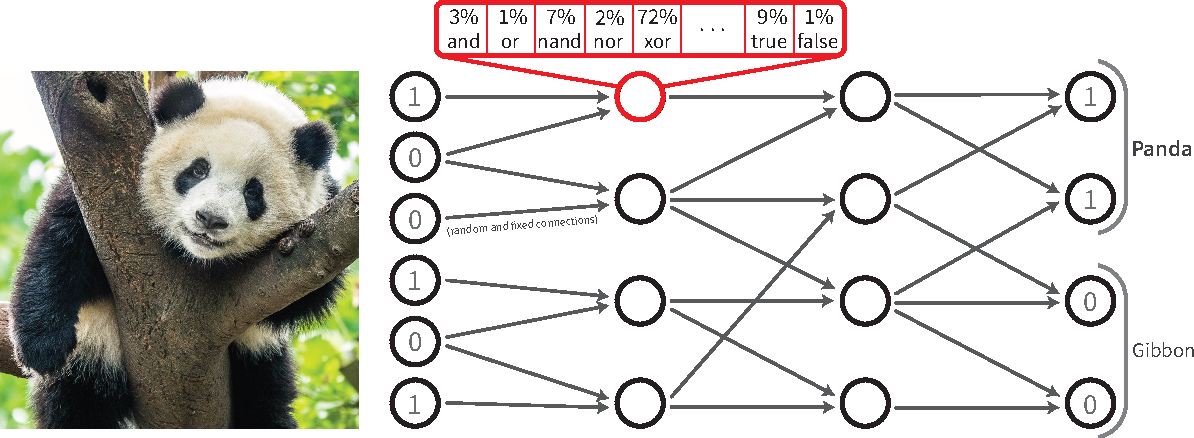
\includegraphics[width=\linewidth]{plots/LogicGateNetOverview_1.pdf}
        \captionof{figure}{An example of a DLGN structure\cite{petersen2022difflogic}}
        \label{fig:logic_gate_network}
    \end{minipage}

\end{minipage}


Let \(x \in \{0,1\}^{d}\) denote a binary input vector, where \(d \in \mathbb{N}\) is the number of input features. The model consists of \(m \in \mathbb{N}\) logic layers followed by a final aggregation stage producing class scores for \(k \in \mathbb{N}\) output classes. The full classifier implements a function
\[
f : \{0,1\}^{d} \rightarrow \mathbb{R}^{k}.
\]

In contrast to ANNs, each neuron of a DLGN consists of a set of every possible binary boolean funtion $\mathcal{G} = \{g_1,\ldots,g_{16}\}$ and corresponding learnable weights 

\[W_j^{(\ell)} \in \mathbb{R}^{|\mathcal{G}|} \], 

where \(\ell \in \{1,\ldots,m\}\) index the logic layers, \(j \in \{1,\ldots,d_\ell\}\) indexes a neuron in the layer and \(d_\ell \in \mathbb{N}\) denotes the number of neurons in layer $\ell$. In order to produce a categorical distribution $\pi_j^{(\ell)}$ a softmax function is applied:

\[
\pi_j^{(\ell)}(g)
=
\frac{
\exp\!\left(
W_{jg}^{(\ell)}
\right)
}{
\sum_{g' \in \mathcal{G}}
\exp\!\left(
W_{jg'}^{(\ell)}
\right)
}.
\]

The output of neuron \(j\) is computed as
\[
\tilde{h}_j^{(\ell)}
=
\sum_{g\in\mathcal{G}}
\pi_j^{(\ell)}(g)\,
g\!\left(z_j^{(\ell)}\right),
\]

where $g\!\left(z_j^{(\ell)}\right)$ is the binary output of the operator $g$ and $z_j^{(\ell)} \in \{0,1\}^2$ is a pair of inputs. In the standart DLGN formulation the connectivity pattern is fixed before the training and is not optimized.

The neurons are stacked into layers in the matter of a classical ANN. Denote the input and output of layer \(\ell\) as $h^{(\ell-1)} \in [0,1]^{d_{\ell-1}}$ and \(h^{(0)} := x\), the input vector of the model. Each vector \(h^{(\ell)}\) contains the outputs of all neurons in layer \(\ell\).

After the final logic layer, neuron outputs are aggregated to produce  (TODO woher) class logits $o(x) \in \mathbb{R}^{k}$. Predicted class probabilities are also obtained using the softmax function,
\[
p(c \mid x)
=
\frac{
\exp(o_c(x))
}{
\sum_{c'=1}^{k}
\exp(o_{c'}(x))
}.
\]


Training minimises the cross-entropy objective
\[
\mathcal{L}
=
-
\sum_{i=1}^{N}
\sum_{c=1}^{k}
\mathbb{I}
[
y_i=c
]
\log
p(c\mid x_i),
\]
where $N$ denotes the number of observations in the training set and $x_i$ - the $i$-th observation. Parameters are optimised using gradient-based methods.

After training, each neuron's soft gate distribution is converted into a deterministic logical operator. For neuron \(j\) in layer \(\ell\), the selected gate is
\[
g_j^{(\ell)*}
=
\arg\max_{g\in\mathcal{G}}
W_{jg}^{(\ell)}.
\]
By recursively selecting the gates a usable circuit is learned.



\clearpage
\section{Methodology}
\label{sec:methodology}

Our approach is based on the idea that methodologies used in logic-based deep learning can be adapted for one-class classification tasks on graph data and, consequently, for graph anomaly detection. This research is limited to OCGIN models and loss-based constraint learning. The motivation behind this approach is to investigate how anomaly detection models respond when the loss function is influenced by constraint values. More specifically, we aim to examine whether models can achieve improved representations by enforcing entities to be positioned closer to or farther away from the center of the hypersphere. 

Due to lack of data the logic used in the loss will be generated automatically. The constraints should be capable of capturing both node-level structural information and aspects of the overall graph representation.

In this chapter, we describe the challenges associated with automatic constraint generation and its implementation. Afterwards, we discuss the methods used to incorporate these constraints into the loss function of an OCGIN model.

\subsection{Logical Constraint Generation}

Since this study focuses on the general behavior of logical constraints without posession of domain-specific semantic knowledge about the data, it was necessary to develop a method for automatically generating constraints.

One of the main challenges, which will be discussed in the next chapter, is the limited availability of anomaly detection datasets. Furthermore, the few existing datasets rarely provide predefined logical constraints that could be directly incorporated into the learning process. Our approach to an automatic generation pipeline is based on applying decision trees.

Decision trees naturally generate logical statements containing operators such as \texttt{OR}, \texttt{AND}, \texttt{<}, and \texttt{\(\geq\)}. This makes them particularly suitable for handling continuous and binary features, and their combinations. Categorical features and can be converted into binary by using one-hot-encoding. Furthermore, the interpretability of this method allows a more detailed analysis of the results. We train a decision tree on structural graph features and convert each root-to-leaf path into a logical rule.

To also obtain features that capture structural properties of graphs, we compute a set of hand-crafted descriptors before training the decision tree. These features are meant to capture not only the node features but also the graph structure.

For each node $v \in V$, in a graph $G = (V, E)$, where $d_\text{in}$ denotes the dimensionality of the input space we extract:

\begin{enumerate}
  \item Raw node features: The original attribute vector $\mathbf{x}_v \in \mathbb{R}^{d_{\text{in}}}$, where each dimension is treated as a separate feature.
  
  \item Node degree: The number of verticies, connected to a node as:
  
  \begin{equation}
  \deg(v) = |\mathcal{N}(v)|.
  \end{equation}
  
  \item Local clustering coefficient: The fraction of possible triangles through $v$ that actually exist:
  
  \begin{equation}
  \text{CC}(v) = \frac{2 \cdot |\{ (u,w) \in E : u,w \in \mathcal{N}(v) \}|}{\deg(v) \cdot (\deg(v) - 1)},
  \end{equation}
  
  where the numerator counts edges between neighbors of $v$.
\end{enumerate}

Each feature dimension is assigned a numeric index. The resulting feature matrix $\mathbf{X} \in \mathbb{R}^{m \times p}$, where $m$ is the number of samples (nodes or graphs) and $p$ is the total number of feature dimensions, is the input to the decision tree.

Once the tree is trained, every root-to-leaf path defines a conjunctive rule. A path of length $L$ to a leaf $j$ produces the rule:

\begin{equation}
r_j: \bigwedge_{\ell = 1}^{L} \bigl( x_{f_\ell} \bowtie_\ell \theta_\ell \bigr) \implies \hat{y}_j,
\end{equation}

where $\bowtie_\ell \in \{\leq, >\}$ is the comparison operator and $\hat{y}_j$ is the majority class of the leaf. The conjunction of all conditions along the path must hold for a sample to be assigned to that leaf's class. The complete decision tree represents a disjunction of such conjunctive rules:

\begin{equation}
\hat{y}(\mathbf{x}) = \bigvee_{j \in R_{\text{ind}}} r_j(\mathbf{x}),
\end{equation}

where $R_{\text{ind}}$ is the set of all available root-toleaf paths.

Each rule is serialized into a JSON structure:

\begin{verbatim}
{
  "conditions": [
    {"feature_index": 729, "op": "<=", "threshold": 0.0},
    {"feature_index": 1263, "op": "<=", "threshold": 0.0}
  ],
  "predicted_class": 1,
  "meta": {"depth": 2, "y_label_number": "20 v.s. 45"}
}
\end{verbatim}

The \texttt{feature\_index} refers to the column index in the feature matrix $\mathbf{X}$, \texttt{op} is the comparison operator, and \texttt{threshold} is the split value. The \texttt{predicted\_class} indicates whether samples satisfying this rule are predicted as normal ($0$) or anomalous ($1$). A separate mapping \texttt{additional\_attributes} records which semantic feature each index corresponds to.

To obtain graph-level representations, we employ an aggregation strategy inspired by the global mean pooling operation commonly used in GNNs. In this case, each node inherits the label of its corresponding graph. After training, real valued scores are computed (see section \ref{sec:diff_constraint}) for all nodes within a graph using the node-level scoring procedure. Afterwards they are aggregated by mean to obtain a single graph-level score.

While this approach enables the straightforward generation of logical rules, it uses the greedy generation approach, which can oversee more conplex patterns. Furthermore, the set of logical operators that can be represented is limited to \texttt{\(\geq\)}, \texttt{<}, \texttt{OR}, and \texttt{AND}. Another challenge is related to the evaluation of the decision tree itself, particularly with respect to the quality of the generated splits.

Another difficulty arises from the supervised learning nature of logical rule generation. To ensure a fair comparison, all models must be trained on the same amount of data. However, logic-based models may gain an advantage from the decision-tree structure itself, which could introduce bias into the evaluation.
    
\subsection{Differentiable Constraint Evaluation}
\label{sec:diff_constraint}

The logical rules are discrete and non-differentiable. To use them within a gradient-based training, we convert each rule into a continuous value $L_c \in [0, 1]$ representing the degree to which a sample is anomalous. We propose two alternative approaches: fuzzy logic-based evaluation and distance-based scoring.

\subsubsection{Fuzzy Logic-Based Approach}

The first approach replaces each hard comparison in the decision tree with a sigmoid approximation. The sigmoid relaxation was chosen since it produces a soft boundary and asymptoticly converges to the hard predicates. Given a feature value $x$, a threshold $t$, the soft variants of the comparisons are defined as:

\begin{equation}
\text{soft\_leq}(x, t) = \sigma \bigl( \gamma \cdot \ (t - x)\bigr),
\qquad
\text{soft\_gt}(x, t) = \sigma\bigl(\gamma \cdot (x - t)\bigr),
\label{eq:soft_comparisons}
\end{equation}

where $\sigma(\cdot)$ is the sigmoid function and $\gamma$ ia a steepness  parameter. As $\gamma \to \infty$, the soft comparisons approach the hard Boolean operators; in practice, $\gamma$ controls the sharpness of the decision boundary.

To combine multiple conditions within a single rule, we use the product t-norm for logical conjunction:

\begin{equation}
\text{soft\_and}(v_1, \dots, v_k) = \prod_{i=1}^{k} v_i,
\end{equation}

and the probabilistic OR for disjunction across rules:

\begin{equation}
\text{soft\_or}(v_1, \dots, v_m) = 1 - \prod_{j=1}^{m} (1 - v_j).
\end{equation}

The product t-norm was selected because it preserves differentiability and provides smooth gradients during optimization. In some cases, the product t-norm is replaced by the minimum t-norm or the Łukasiewicz t-norm due to the rapid vanishing of gradients when a large number of rules is used. However, in this thesis only decision trees with a depth of 2--3 are generated in order to preserve interpretability. Therefore, gradient vanishing is not expected to become a significant issue.

The satisfaction degree of a single rule $r_j$ containing $k$ conditions is therefore:

\begin{equation}
r_j(x) = \prod_{\ell=1}^{k} \text{soft\_cmp}_\ell\bigl(x_{f_\ell}, \theta_\ell\bigr),
\end{equation}

where $\text{soft\_cmp}_\ell \in \{\text{soft\_leg}, \text{soft\_gt}\}$ is the appropriate soft comparison operator for condition $\ell$. The final constraint value for a sample is obtained by aggregating all rules that predict anomalous behavior:

\begin{equation}
L_c(x) = \lambda \cdot \text{soft\_or}\bigl(r_1(x), \dots, r_m(x)\bigr),
\label{eq:fuzzy_constraint}
\end{equation}

where $\lambda$ is a scaling hyperparameter. A value of $L_c$ close to $1$ indicates that the sample strongly satisfies the anomalous rule set, while a value close to $0$ -- normal behavior.

\subsubsection{Distance-Based Scoring Handler}

The second approach evaluates constraints based on the signed margin between a sample and the nearest rule boundary. In contrast to the fuzzy logic formulation, which models rule satisfaction continuously through soft logical operators, this method explicitly considers how far a sample is located from the corresponding decision boundaries. Consequently, samples that satisfy a rule only marginally can be distinguished from samples that lie deeply inside a normal or anomalous region.

The extracted decision tree rules are divided into two groups according to their predicted class:
\begin{itemize}
    \item Normality rules $\mathcal{R}_{\text{norm}}$
    \item Anomaly rules $\mathcal{R}_{\text{anom}}$
\end{itemize}

Each rule consists of a conjunction of threshold conditions of the form
\begin{equation}
x_f \leq \theta
\qquad \text{or} \qquad
x_f > \theta,
\end{equation}
where $f$ denotes the feature index and $\theta$ the corresponding threshold value.

For a single condition $c$, we define the signed margin function
\begin{equation}
d_c(x) = |x_f - \theta|
\end{equation}

The absolute value represents the distance to the corresponding threshold boundary.

Since each rule is formed as a conjunction of conditions, the satisfaction strength of a rule is determined by its weakest satisfied condition, which is equal to the distance between a point and an axis-alighed space. Therefore, the margin of a rule $r$ is defined as

\begin{equation}
d(x, r) =
\min_{c \in r} d_c(x).
\end{equation}

Given a satisfaction function for one condition:

\[
s(x, c) =
\begin{cases}
1, & \text{if } c \equiv (x_f \leq \theta) \text{ and } x_f \leq \theta \text{ or } \\[6pt]
 &  c \equiv (x_f > \theta) \text{ and } x_f > \theta, \\[6pt]
 0 & \text{otherwise},
\end{cases}
\]


a rule is considered satisfied if all of its conditions are fulfilled:

\begin{equation}
\text{satisfies}(x, r) =
\begin{cases}
1, & \text{if } \min_{c \in r} s(x, c) = 1, \\
0, & \text{otherwise}.
\end{cases}
\end{equation}


To obtain a global characterization of the sample with respect to a rule group, the average margin over all rules in the group is computed:

\begin{equation}
\text{group\_dist}(x, \mathcal{R}) =
\frac{\alpha}{|\mathcal{R}|}
\sum_{r \in \mathcal{R}} d(x, r),
\end{equation}

where $\alpha$ is a scaling hyperparameter and $|\mathcal{R}|$ denotes the number of rules in the group.

The relative preference of normality versus anomaly rules is then modeled through the difference

\begin{equation}
\text{group\_diff}(x) =
\text{group\_dist}(x, \mathcal{R}_{\text{norm}})
-
\text{group\_dist}(x, \mathcal{R}_{\text{anom}}).
\end{equation}

Additionally, we define the strongest satisfied rule margins

\begin{equation}
d_{\text{norm}} =
\max_{\{r \in \mathcal{R}_{\text{norm}} | \text{satisfies}(x, r) = 1\} }
d(x, r),
\end{equation}

\begin{equation}
d_{\text{anom}} =
\max_{ \{ r \in \mathcal{R}_{\text{anom}}  | \text{satisfies}(x, r) = 1\} }
d(x, r),
\end{equation}

as well as the distances to the closest rule of the opposite class

\begin{equation}
d_{\text{min,anom}} =
\min_{r \in \mathcal{R}_{\text{anom}}}
|d(x,r)|,
\end{equation}

\begin{equation}
d_{\text{min,norm}} =
\min_{r \in \mathcal{R}_{\text{norm}}}
|d(x,r)|.
\end{equation}

The final score is computed differently depending on the region in which the sample is located.

\begin{enumerate}
    \item \textbf{Normal region:}  
    If the sample satisfies at least one normality rule, i.e.,
    \begin{equation}
    \exists r \in \mathcal{R}_{\text{norm}}
    :
    \text{satisfies}(x,r)=1,
    \end{equation}
    the score is defined as
    \begin{equation}
    \text{score}(x)
    =
    -d_{\text{norm}} \cdot d_{\text{min,anom}}
    +
    \text{group\_diff}(x).
    \end{equation}

    \item \textbf{Anomaly region:}  
    If the sample satisfies at least one anomaly rule, i.e.,
    \begin{equation}
    \exists r \in \mathcal{R}_{\text{anom}}
    :
    \text{satisfies}(x,r)=1,
    \end{equation}
    the score becomes
    \begin{equation}
    \text{score}(x)
    =
    d_{\text{anom}} \cdot d_{\text{min,norm}}
    +
    \text{group\_diff}(x).
    \end{equation}

    \item \textbf{Grey zone:}  
    If the sample satisfies neither a normality nor an anomaly rule, it is considered to lie in an uncertain region between the extracted logical partitions. In this case, only the group distance difference contributes:
    \begin{equation}
    \text{score}(x)
    =
    \text{group\_diff}(x).
    \end{equation}
\end{enumerate}

The multiplicative margin terms emphasize samples that are located deeply inside one rule region and are far away from rules of the opposite class. Consequently, the confidence increases nonlinearly with increasing separation between normal and anomalous regions. In contrast, samples located in the grey zone are modeled only through the linear group distance difference.

Finally, the raw score is transformed into a bounded anomaly score using a sigmoid function

\begin{equation}
L_c(x) = \lambda \sigma(\text{score}(x)),
\end{equation}

and a scaling hyperparameter $\lambda$ mapping the output onto the interval $[0,1]$. Higher values of $L_c(x)$ therefore indicate stronger agreement with the extracted anomaly rules, while lower values correspond to stronger agreement with normality rules.

\subsection{Constraint Integration into the Loss Function}

Once constraint values $L_c$ have been computed for each sample, they must be incorporated into the training objective. The base loss of the OCGIN model is the Deep SVDD objective, which minimises the squared distance between graph or node embeddings $z_i$ and a learned center $c$:

\begin{equation}
\mathcal{L}_{\text{SVDD}} = \frac{1}{N} \sum_{i=1}^{N} \| z_i - c \|^2,
\end{equation}

where $N$ is the number of nodes or graphs. We propose three strategies for combining this base loss with the constraint values. Each strategy encodes a different assumption about how the model should respond to samples that violate the logical rules.

\paragraph{Additive Constraint Loss.}

The simplest approach adds the mean constraint value as an additional penalty term:

\begin{equation}
\mathcal{L}_{\text{total}} = \frac{1}{N} \sum_{i=1}^{N} \| z_i - c \|^2 \;+\; \frac{1}{N} \sum_{i=1}^{N} L_c^{(i)}.
\end{equation}

This formulation treats the constraint penalty as independent of the embedding distance. Samples that violate the rules receive an additional loss contribution regardless of how far they are from the center. The effect is that the model is encouraged to find embeddings that simultaneously minimise the hypersphere radius and satisfy the logical constraints.

\paragraph{Weighted Constraint Loss.}

The second approach weights the SVDD loss of each sample by its constraint value:

\begin{equation}
\mathcal{L}_{\text{total}} = \frac{1}{N} \sum_{i=1}^{N} \| z_i - c \|^2 \cdot \bigl(1 + L_c^{(i)}\bigr).
\label{eq:loss_weight}
\end{equation}

Here, samples with high constraint values (i.e., samples that likely violate the logical rules) contribute more to the total loss. This amplifies the gradient signal for suspicious samples, pushing their embeddings further away from the center. Normal samples with $L_c \approx 0$ are unaffected.

\paragraph{Supression Loss}

The third approach is the inverse of weighting:

\begin{equation}
\mathcal{L}_{\text{total}} = \frac{1}{N} \sum_{i=1}^{N} \| z_i - c \|^2 \cdot \bigl(1 - L_c^{(i)}\bigr).
\label{eq:loss_ignore}
\end{equation}

Samples with high constraint values are down-weighted, effectively causing the model to ignore them during training. The motivation behind this strategy is that samples flagged by the logical rules may be ambiguous or mislabeled; reducing their influence on the loss may lead to a more robust hypersphere representation. However, this comes at the risk of discarding informative training signals.

\subsection{Loss-Only and Constraint-Aware Inference Model Variants}

Beyond how constraints are integrated into the loss, we distinguish two fundamental model paradigms based on whether the constraints also influence the anomaly score at inference time.

\subsubsection{Pure Loss-Based Models}

In the loss-only variant, the constraint values are used exclusively during training. At inference time, the anomaly score reverts to the standard OCGIN formulation:

\begin{equation}
a_i = \| z_i - c \|^2.
\label{eq:score_loss_only}
\end{equation}

The logical constraints therefore serve purely as a regularisation mechanism that shapes the embedding space during training. This approach is simpler and ensures that the test-time behaviour is identical to the baseline OCGIN, making it easier to isolate the effect of constraint-based regularisation.

\subsubsection{Constraint-Aware Inference Models}

In this variant, the constraints are also applied during inference by incorporating them into the anomaly score. The three integration strategies are applied identically to how they were used in the loss:

\begin{align}
a_i &= \| z_i - c \|^2 + L_c^{(i)} \quad &&\text{(additive)}, \\
a_i &= \| z_i - c \|^2 \cdot \bigl(1 + L_c^{(i)}\bigr) \quad &&\text{(weighting)}
\label{eq:scores_forecast}
\end{align}

This means that the constraints must be available at test time.

While the suppression-based strategy reduces the influence of suspicious samples during training, its usage in iference time is incoherent. 

\clearpage
\subsection{Logic Gate Networks}

Many graph datasets used in this work contain predominantly categorical or binary features, such as bag-of-words representations in citation networks. For such features, decision trees may produce suboptimal partitions due to their reliance on threshold-based splits. As an alternative, we employ logic gate networks~\cite{petersen2022difflogic}, which learn Boolean formulas directly from binary data through differentiable optimization.

\subsubsection{Architecture}

A logic gate network consists of differentiable layers that learn combinations of Boolean gates. Each neuron in a logic layer selects a subset of its inputs and learns which Boolean function to apply. The full model used in this work is defined as

\[
\text{Model} = \texttt{GroupSum} \circ \texttt{LogicDense}^{(2)} \circ \texttt{LogicDense}^{(1)} \circ \texttt{FixedBinarization},
\]

where the input is first binarized, passed through two logic dense layers, and aggregated into class scores.

\paragraph{LogicDense Layer.}
A LogicDense layer with input dimension $d_{\text{in}}$ and output dimension $d_{\text{out}}$ is parameterized by a connection pattern and a set of gate type logits. Each output neuron connects to exactly $r$ input slots, where $r$ is the LUT rank. The connections are given by

\[
C \in \{0,\dots,d_{\text{in}}-1\}^{d_{\text{out}} \times r},
\]

where $C_{j\ell}$ specifies which input feeds into slot $\ell$ of neuron $j$. The LUT rank is chosen such that $d_{\text{out}} \cdot r \geq d_{\text{in}}$, ensuring full input coverage.

For each input slot, the layer learns a categorical distribution over a set of Boolean gate types $\mathcal{G}$. In the \emph{raw} parametrization used here, each slot is parameterized by $|\mathcal{G}| = 16$ learnable logits, representing all possible Boolean functions of two inputs. Let $W_{j\ell} \in \mathbb{R}^{16}$ denote the logits for slot $\ell$ of neuron $j$. During training, the output of the neuron is a differentiable relaxation:

\[
P(G_{j\ell} = g) = \frac{\exp((W_{j\ell})_g)}{\sum_{g'=1}^{16} \exp((W_{j\ell})_{g'})},
\qquad
\tilde{h}_j = \sum_{\ell=1}^{r} \sum_{g=1}^{16} P(G_{j\ell} = g) \cdot g(b_{C_{j\ell}}).
\]

After training, the model is discretized by replacing the probability distribution with the most probable gate:

\[
g_{j\ell}^* = \arg\max_{g \in \{1,\dots,16\}} (W_{j\ell})_g,
\]

and evaluating the network using hard Boolean logic. The resulting discretized network is a pure Boolean circuit that can be executed efficiently.

For the purpose of rule extraction, each learned gate is mapped to one of four semantic types relevant to constraint generation TODO there are more:

\[
\mathrm{gate}(W_{j\ell}) \in \{\mathrm{INPUT}, \mathrm{NOT\_INPUT}, \mathrm{AND}, \mathrm{OR}\},
\]

where $\mathrm{INPUT}$ passes the feature value unchanged, $\mathrm{NOT\_INPUT}$ negates it, AND combines multiple conditions conjunctively, and OR introduces disjunctive alternatives.

\paragraph{GroupSum.}
The final layer aggregates neuron outputs into per-class logits. Given $k$ classes and $n$ neurons divided into $k$ groups, the output for class $k$ is

\[
y_k = \frac{1}{\tau} \sum_{j \in \text{group}(k)} h_j,
\]

where $\tau$ is a temperature parameter that scales the output range.

\subsubsection{Training}

The logic gate network is trained end-to-end using the cross-entropy loss and the Adam optimizer. During training, the continuous relaxation allows gradient flow through the gate selection mechanism, enabling the network to learn which Boolean functions are most predictive. At inference time, the model is discretized, and only the most probable gates are retained. The resulting network captures logical combinations of binary features that discriminate between normal and anomalous samples.

\subsubsection{Rule Extraction}

After training and discretization, we extract logical rules from the learned gates and connections. The extraction proceeds by traversing the network from output back to input.

For each output neuron in the second LogicDense layer, we determine its predicted class from the gate type of each of its $r$ slots. $\mathrm{INPUT}$ and $\mathrm{AND}$ gates indicate a positive prediction (anomalous), while $\mathrm{NOT\_INPUT}$ indicates a negative prediction (normal). For each such slot, we trace its connection back to a hidden neuron in the first layer and examine that hidden neuron's input slots. Each slot contributes a condition:

\[
\text{condition}(g, f) =
\begin{cases}
x_f > 0.5, & \mathrm{if } g \in \{\mathrm{INPUT}, \mathrm{AND}\}, \\[4pt]
x_f \leq 0.5, & \mathrm{if } g = \mathrm{NOT\_INPUT}.
\end{cases}
\]

Slots classified as OR are extracted as separate disjunctive rules rather than conjoined with the other conditions.

A single path from input features to an output class defines a conjunctive rule:

\[
r_j: \bigwedge_{\ell=1}^{L} \bigl( x_{f_{j\ell}} \bowtie_{j\ell} 0.5 \bigr) \implies \hat{y}_j,
\]

where $\bowtie_{j\ell} \in \{\leq, >\}$ and $\hat{y}_j$ is the predicted class. The complete model represents a disjunction of such rules:

\[
\hat{y}(\mathbf{x}) = \bigvee_{j \in R_{\text{logix}}} r_j(\mathbf{x}),
\]

where $R_{\text{logix}}$ is the set of all extracted logic gate rules. Each rule is serialized into the same JSON format used for decision trees, including the feature index, operator, threshold, and predicted class.

\clearpage
\section{Evaluation}
\label{sec:evaluation}

In this chapter we evaluate the proposed methods on Graph datasets. We first describe the experimental setup including used data, hyperparameters and a detailed flow of a single experiment. Then we evaluate those results using a variety of metrics as ROC-AUC.

\subsection{Experimental setup}

Since this work is primarily theoretical, we chose to evaluate each model across a diverse set of datasets from different domains, using a wide range of hyperparameter configurations.

\subsubsection{Datasets}

To evaluate the proposed methods under different structural conditions, experiments were conducted on a diverse collection of graph datasets originating from multiple application domains. The selected datasets cover citation networks, co-authorship graphs, web page networks, molecular graphs, protein structures, and computer vision tasks. This diversity was intentionally chosen to evaluate how the proposed mechanisms affect the learning process across different graph characteristics and semantic domains.

All chosen datasets are also available from as pytorch datasets, which makes their implementation straightforward.

\paragraph{Planetoid Datasets.}

The \texttt{Cora}, \texttt{CiteSeer}, and \texttt{PubMed} datasets belong to the Planetoid benchmark collection. In these datasets, nodes represent scientific publications and edges correspond to citation relationships between papers. Node attributes are represented using bag-of-words feature vectors derived from publication text.

These datasets were selected because they represent sparse real-world human communication networks with high-dimensional node features. Additionally, they are widely used benchmarks in graph representation learning, enabling comparisons with prior work.

\begin{itemize}
    \item \textbf{Cora:} A citation network of machine learning publications divided into multiple research topics.
    
    \item \textbf{CiteSeer:} A citation dataset containing scientific publications from various computer science domains with a relatively sparse graph structure.
    
    \item \textbf{PubMed:} A larger citation network consisting of biomedical research publications related to diabetes.
\end{itemize}

\paragraph{Coauthor Dataset.}

The \texttt{CS} dataset from the Coauthor benchmark collection models collaboration networks between authors in the field of computer science. Nodes represent authors and edges indicate co-authorship relations.

This dataset was chosen because co-authorship networks exhibit structural properties that differ significantly from citation graphs, including denser local communities and stronger clustering behaviour. Consequently, it provides a complementary graph topology for evaluating the robustness of the constraint extraction methods.

\paragraph{Amazon Dataset.}

The \texttt{Photo} dataset from the Amazon benchmark collection represents a product co-purchasing network. Nodes correspond to products, while edges indicate that two products are frequently purchased together.

This dataset introduces a commercially oriented graph structure that differs from academic citation networks. The dataset was selected to evaluate whether the proposed constraints remain effective in recommendation-style graph environments with different feature distributions and connectivity patterns.

\paragraph{WebKB Datasets.}

The \texttt{Texas}, \texttt{Cornell}, and \texttt{Wisconsin} datasets originate from the WebKB benchmark collection. Nodes represent web pages and edges correspond to hyperlinks between pages within university web domains.

These datasets were selected because they contain comparatively small and heterogeneous graph structures with irregular connectivity patterns. Their inclusion allows evaluating the behaviour of the proposed methods under low-data conditions and structurally noisy environments.


\paragraph{Bioinformatics Datasets.}

The \texttt{MUTAG}, \texttt{AIDS}, \texttt{DHFR}, \texttt{ENZYMES}, and \texttt{PROTEINS} datasets represent molecular and biological graph structures. In these datasets, nodes typically correspond to atoms or biological components, while edges represent chemical bonds or interactions.

These datasets were chosen because they contain highly structured graph topologies with strong local dependencies, making them well suited for evaluating whether the methods can capture meaningful structural regularities.

\begin{itemize}
    \item \textbf{MUTAG:} A molecular graph dataset describing mutagenic aromatic and heteroaromatic nitro compounds.
    
    \item \textbf{AIDS:} A molecular dataset containing chemical compounds evaluated for anti-HIV activity.
    
    \item \textbf{DHFR:} A dataset of molecular compounds related to dihydrofolate reductase inhibition.
    
    \item \textbf{ENZYMES:} A protein structure dataset where graphs represent tertiary enzyme structures categorized into enzyme classes.
    
    \item \textbf{PROTEINS:} A dataset consisting of protein structures represented as graphs derived from spatial and sequential relationships.
\end{itemize}

\paragraph{Computer Vision Datasets.}

The \texttt{COIL-RAG} and \texttt{MSRC\_21} datasets originate from computer vision tasks in which images are transformed into graph representations.

These datasets were selected to evaluate the proposed methods on graph structures generated from visual information rather than naturally relational data. Consequently, they provide an additional level of diversity in graph topology and feature semantics.

\begin{itemize}
    \item \textbf{COIL-RAG:} A graph-based version of the COIL object image dataset, where image regions are represented as attributed relational graphs.
    
    \item \textbf{MSRC\_21:} A scene classification dataset represented as graphs constructed from segmented image regions and their spatial relationships.
\end{itemize}









\subsection{Experimental Hyperparameter Configuration}

The experimental evaluation compared baseline OCGIN models with the proposed logic-enhanced variants under identical architectural conditions. To ensure fair comparison, each logic-enhanced model used the same backbone configuration as its corresponding baseline OCGIN model.

The hyperparameter search consisted of two categories:

\begin{enumerate}
    \item baseline OCGIN hyperparameters, defining the embedding architecture;
    \item constraint-specific hyperparameters, controlling logical rule extraction and integration.
\end{enumerate}

For each baseline architecture, all combinations of constraint-related hyperparameters were evaluated independently, enabling direct comparison between the baseline model and multiple logic-enhanced variants sharing the same embedding space dimentions.

Several optimization parameters were kept fixed across all experiments to maintain a computationally feasible search space. Both node-level and graph-level experiments used the training configuration shown in Table~\ref{tab:fixed_hp}.



\begin{table}[h]
\centering
\caption{Fixed training hyperparameters used in all experiments.}
\label{tab:fixed_hp}
\begin{tabular}{lc}
\toprule
Hyperparameter & Value \\
\midrule
Learning rate & $10^{-3}$ \\
Training epochs & 50 \\
Batch size & 32 \\
Sigmoid steepness parameter & 1\\
Decision tree depth & 3 \\
\bottomrule
\end{tabular}
\end{table}


The evaluated hyperparameter ranges are summarized in Table~\ref{tab:search_space}. Hidden dimensionalities and layer counts were selected to examine behaviour across both compact and high-capacity embedding spaces.

\begin{table*}[h]
\centering
\caption{Hyperparameter search space.}
\label{tab:search_space}
\begin{tabular}{lll}
\toprule
Category & Hyperparameter & Evaluated values \\
\midrule
\multirow{2}{*}{Baseline OCGIN}
& Hidden dimension
& $\{4,8,16,32,64,128,256,512\}$ \\

& Number of GNN layers
& $\{2,3,4,5\}$ \\

\midrule
\multirow{5}{*}{Constraint-specific}
& Constraint scaling factor $\alpha$
& $\{1,0.5,0.1,0.01,0.001\}$ \\

& Constraint handler
& \{fuzzy logic, distance-based\} \\

& Integration strategy
& \{additive, weighting, suppression\} \\

& Integration type
& \{training-only, inference-time\} \\
\bottomrule
\end{tabular}
\end{table*}




\subsection{Experimental Procedure}

The complete experimental workflow was executed separately for every dataset and hyperparameter configuration. For each experiment, the following procedure was executed:

\begin{enumerate}
    \item \textbf{Dataset partitioning}

    The dataset was randomly divided into four subsets:

    \begin{itemize}
        \item \textbf{Training set}: used for OCGIN optimization and containing only normal samples;
        \item \textbf{Validation set}: used for anomaly threshold selection and containing both normal and anomalous samples;
        \item \textbf{Test set}: reserved exclusively for final evaluation;
        \item \textbf{Tree set}: used solely for training the decision tree responsible for logical rule extraction.
    \end{itemize}

    The separation between the training and tree subsets prevented logical rules from being extracted directly from the data used to optimize the embedding model.

    The separation was also done in baseline models to keep the number of datapoints used for training equal. 

    \item \textbf{Logical rule extraction}

    A decision tree was trained on the tree subset using the handcrafted structural features introduced previously. Depending on the experiment, either node-level or graph-level descriptors were employed.

    Logical constraints were generated by converting each root-to-leaf decision path into a conjunction of threshold conditions. The resulting rule set was serialized and provided to the selected differentiable constraint handler. This step was ommited for baseline models.

    \item \textbf{Model initialization}

    The OCGIN backbone was initialized using the selected architectural hyperparameters.

    Following the standard Deep SVDD initialization procedure, the hypersphere center was computed as the mean embedding of normal training samples produced by the randomly initialized network.

    \item \textbf{Model training}

    The model was optimized either using the selected constraint integration strategy or the classical DeepSVVD objective.

    \item \textbf{Threshold selection}

    After training, anomaly scores were computed on the validation set. The final decision threshold was selected using Youden's \(J\) statistic.

    \item \textbf{Final evaluation}

    The trained model was evaluated on the test set using the threshold selected on the validation data.

    Performance was assessed using standard anomaly detection metrics, including ROC-AUC, balanced accuracy, precision, and recall.
\end{enumerate}


\subsection{Used Software}

All experiments in this thesis were implemented using Python~\cite{python} (Version~3.12). The deep learning framework PyTorch~\cite{paszke2019pytorch} (Version~2.5) with CUDA~\cite{nvidia2023cuda} 12.1 support was used for model implementation and GPU-accelerated training. Graph neural network operations were implemented using PyTorch Geometric~\cite{fey2019pytorchgeometric} (Version~2.7.0). Additional graph-level anomaly detection models were evaluated using the PyGOD library~\cite{liu2024pygod} (Version~1.1.0). The logic gate network experiments used the torchlogix library.

For the constraint generation pipeline, decision trees from scikit-learn~\cite{pedregosa2011scikit} (Version~1.7.2) were employed together with logic gate networks. Scientific computing was performed using NumPy~\cite{harris2020numpy} (Version~2.3.3) and SciPy~\cite{virtanen2020scipy} (Version~1.16.2). Data manipulation and analysis were conducted with pandas~\cite{mckinney2010pandas} (Version~2.3.3). Graph-theoretic computations relied on NetworkX~\cite{hagberg2008networkx} (Version~3.5).

All figures and visualizations were generated using Matplotlib~\cite{hunter2007matplotlib} (Version~3.10.7) and Seaborn~\cite{waskom2021seaborn} (Version~0.13.2). Hyperparameter tuning and model evaluation utilized the metrics module of scikit-learn.



\subsection{Experimental results}

The complete experiment pipeline yielded 27,261 individual trials spanning 15 datasets (8 node-level and 7 graph-level). We organize our analysis around five key questions: (1) How do the six model variants compare overall? (2) Do loss-only models differ from inference models? (3) How does the constraint strength parameter $\lambda$ affect performance? (4) Do the constraint handlers perform differently? (5) Which model achieves the best configuration per dataset? All statistical comparisons were performed using the two-sided Mann-Whitney U test, a non-parametric test that does not assume normality of the underlying distributions. This choice is appropriate for comparing ROC-AUC scores across independent hyperparameter configurations, where the distributions may be skewed or multimodal. We report the median alongside the mean for each group, as the median is more robust to outliers. Under a Bonferroni correction for the 15 pairwise tests the significance threshold becomes $\alpha \approx 0.003$; all loss-only vs baseline comparisons remain non-significant and all Inference-Add comparisons remain significant at this threshold.

\subsubsection{Overall Model Comparison}

\begin{figure}[H]
    \centering
    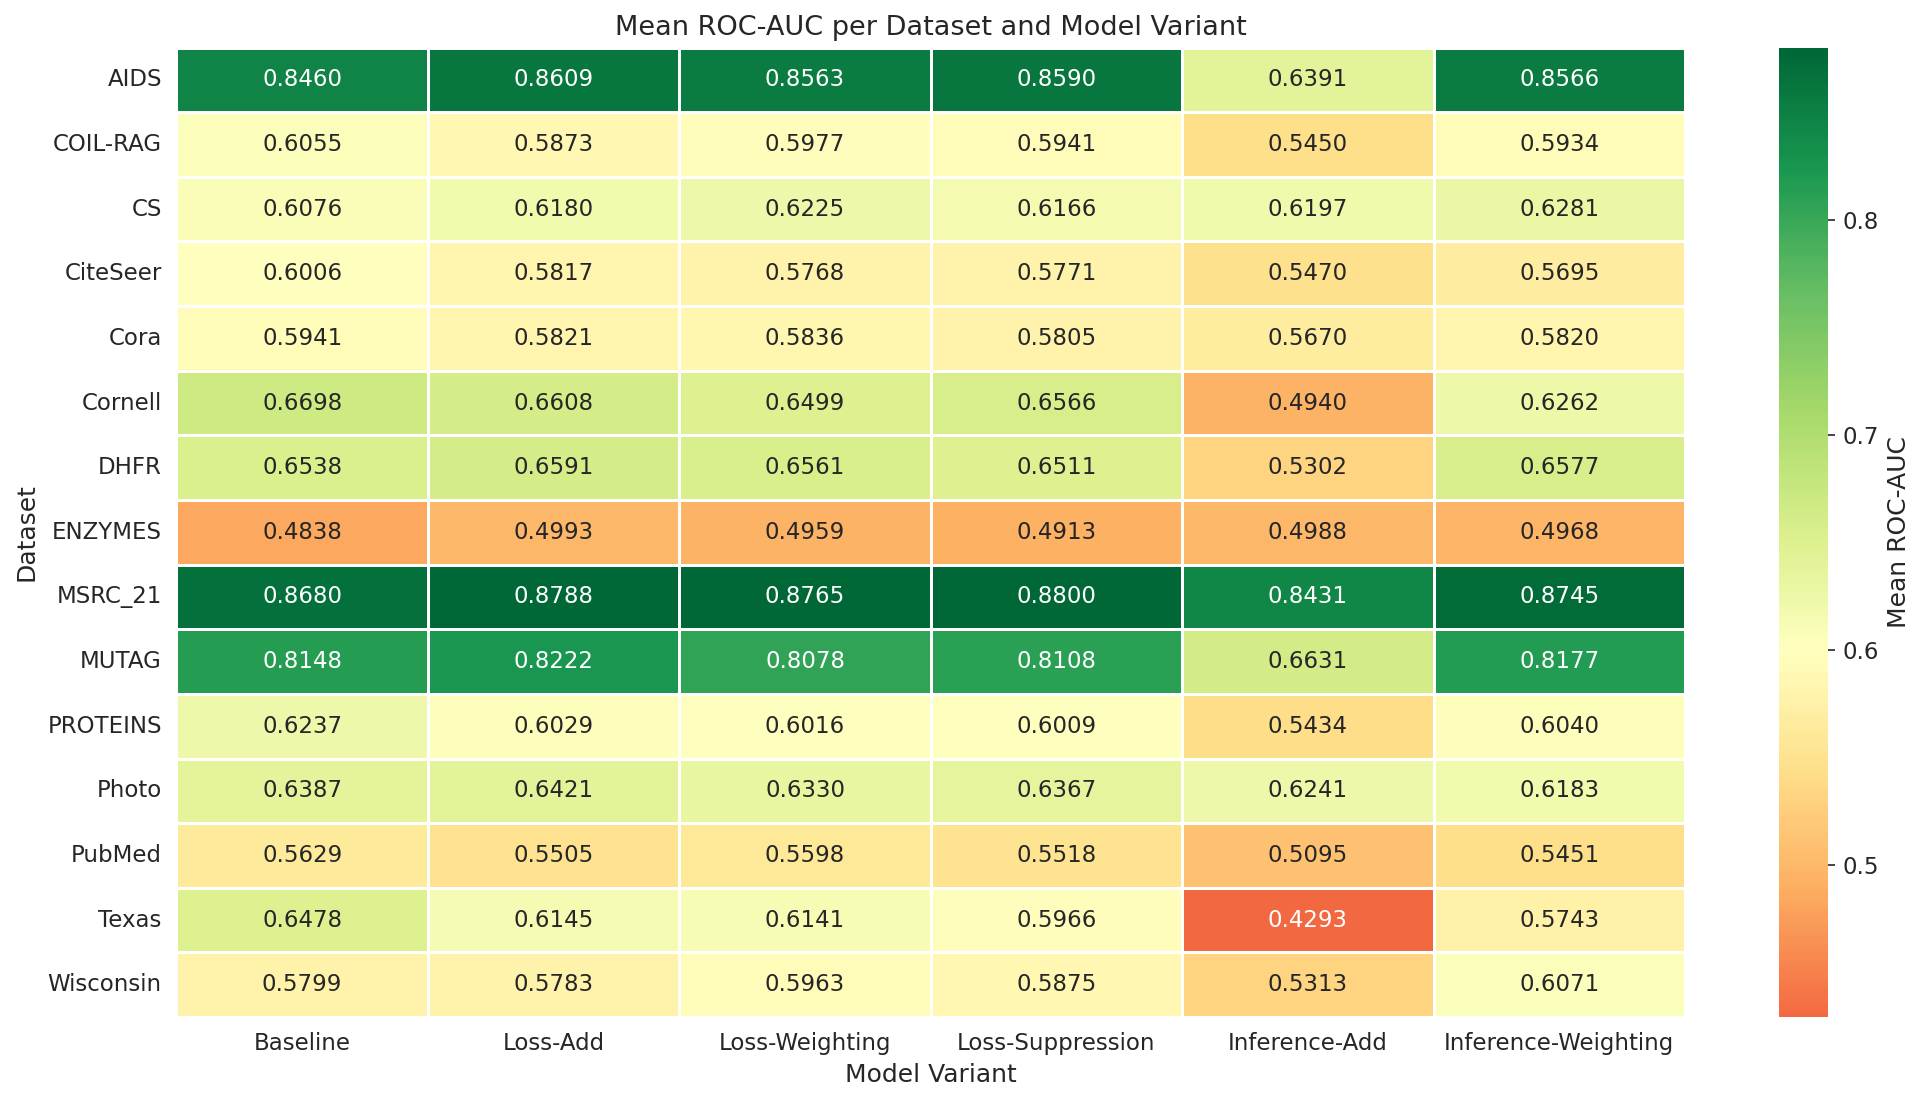
\includegraphics[width=\textwidth]{plots/model_ranking_heatmap.png}
    \caption{Mean ROC-AUC per dataset and model variant.}
    \label{fig:model_ranking}
\end{figure}

Figure~\ref{fig:model_ranking} presents the average ROC-AUC ranking of all six model variants across all datasets. The baseline and loss-only models (Loss-Add, Loss-Weighting, Loss-Suppression) occupy the top positions with near-identical ranks. The inference variants, particularly Inference-Add, rank substantially worse.

The boxplot in Figure~\ref{fig:roc_boxplot_node} shows the distribution of ROC-AUC scores for node-level prediction across model variants. The corresponding graph-level boxplot (omitted for brevity) exhibits the same pattern. Decision tree depth (3 or 4) showed negligible effect on all metrics; results are aggregated across both depths.

\begin{figure}[H]
    \centering
    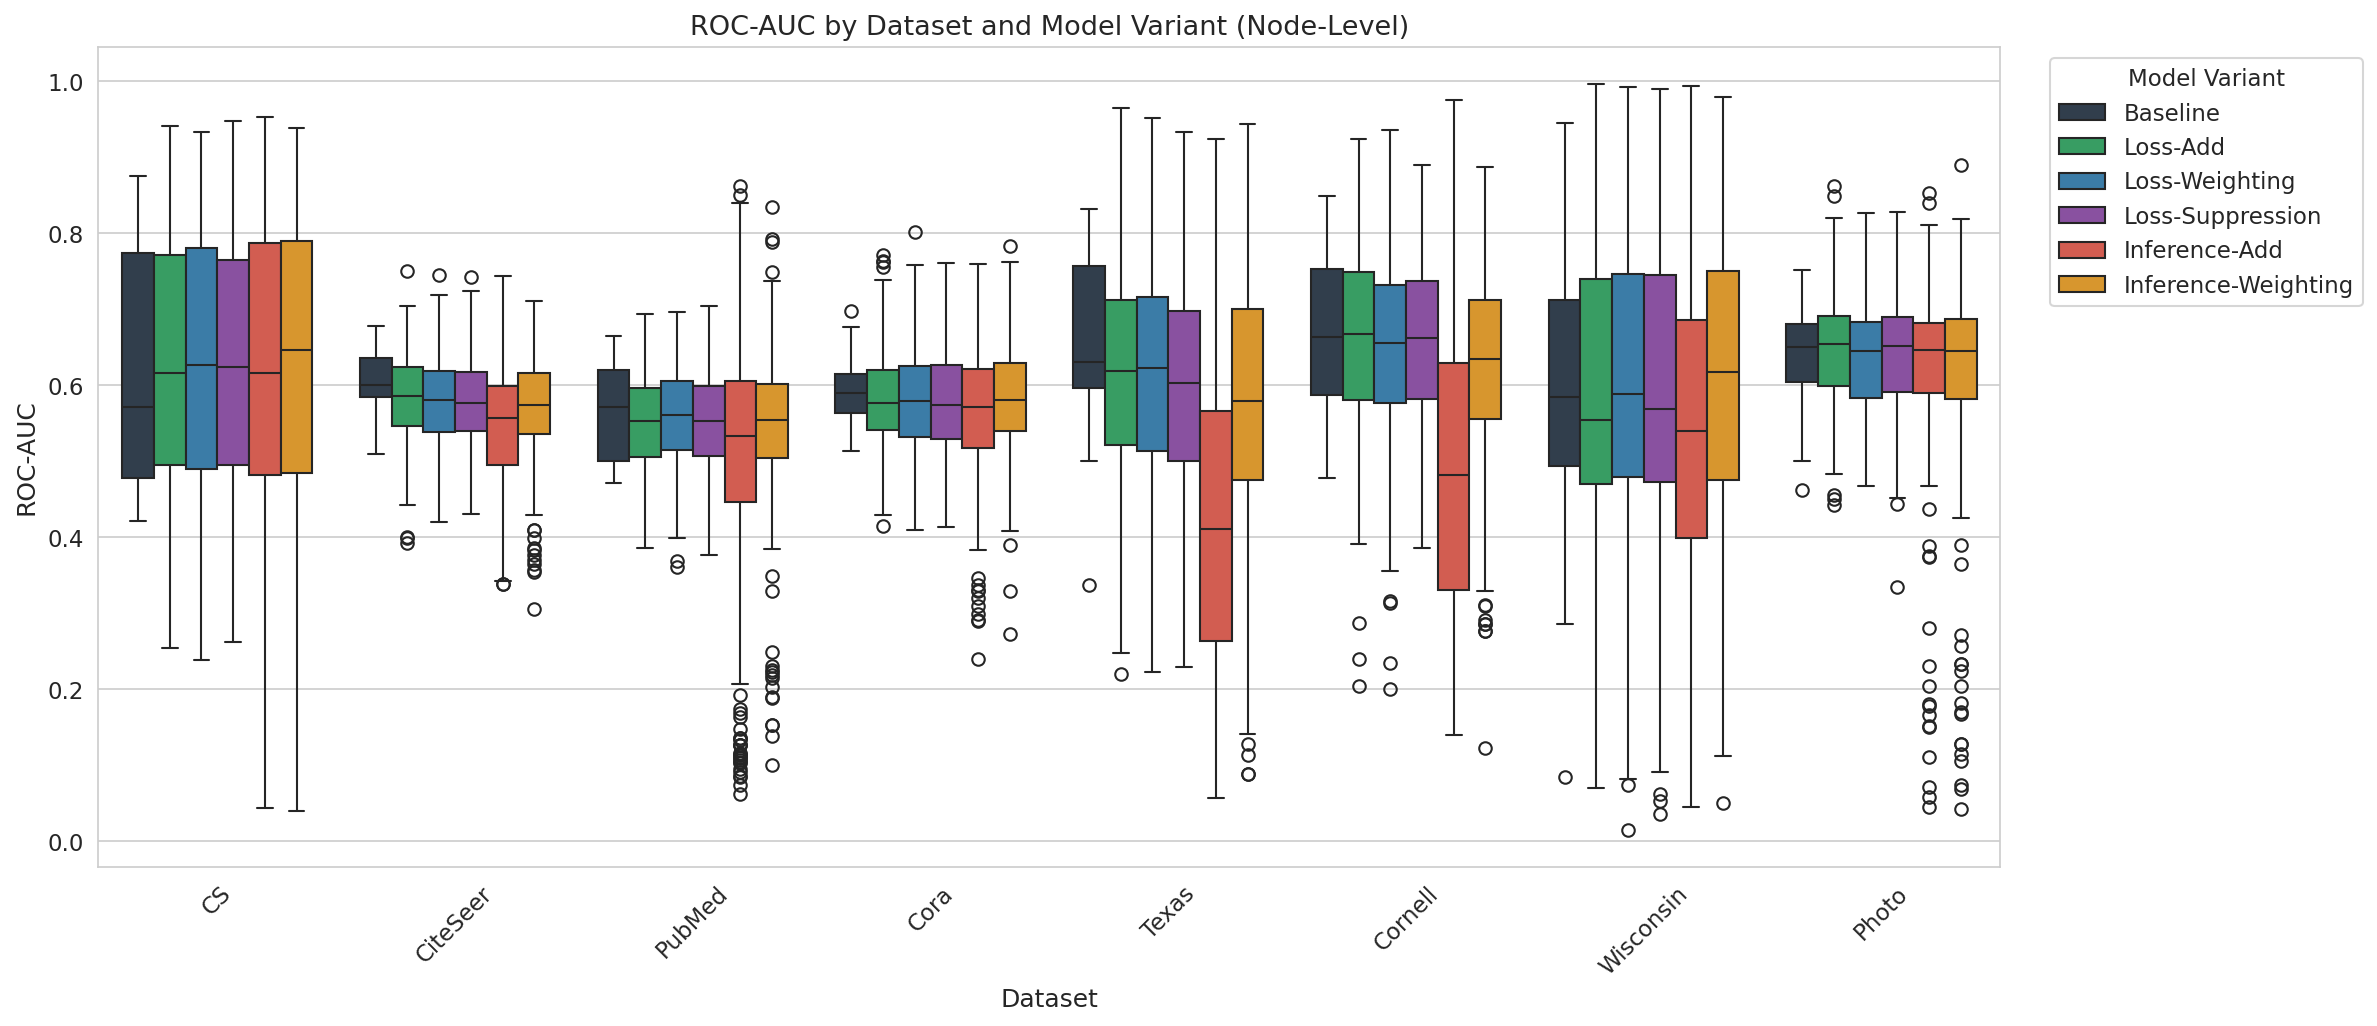
\includegraphics[width=\textwidth]{plots/node_roc_auc_boxplot.png}
    \caption{ROC-AUC distribution for node-level prediction across model variants. The central line marks the median, boxes show the interquartile range, and whiskers extend to 1.5$\times$IQR.}
    \label{fig:roc_boxplot_node}
\end{figure}

The baseline has only 270 configurations compared to 5,400 for each constraint variant, which likely contributes to the larger observed variance. For every logical model variant, 5,400 configurations were evaluated, compared to only 270 baseline configurations. Apart from these datasets, the baseline achieves higher median ROC-AUC than any constraint variant on CiteSeer and Texas, though the overall difference is not significant ($p > 0.40$). The Inference-Add model showed only somewhat worse results on most datasets, but failed deeply on Texas and Cornell.

To verify these observations, we performed pairwise Mann-Whitney U tests between all model variants. The results confirm that none of the loss-only models differ significantly from the baseline (Loss-Add: $p = 0.58$, Loss-Weighting: $p = 0.63$, Loss-Suppression: $p = 0.40$). Inference-Add, however, is significantly worse than every other model (all $p < 10^{-10}$), including Inference-Weighting ($p < 10^{-10}$). Inference-Weighting does not differ significantly from the baseline ($p = 0.38$) or from any of the loss-only models (all $p > 0.23$).

\subsubsection{Loss-Only vs.\ Constraint-Aware Inference}

A central design question is whether constraints should affect only training (loss-only) or also influence the decision at inference time (constraint-aware). Figure~\ref{fig:loss_vs_inference_node} compares these two approaches for each model variant.

\begin{figure}[H]
    \centering
    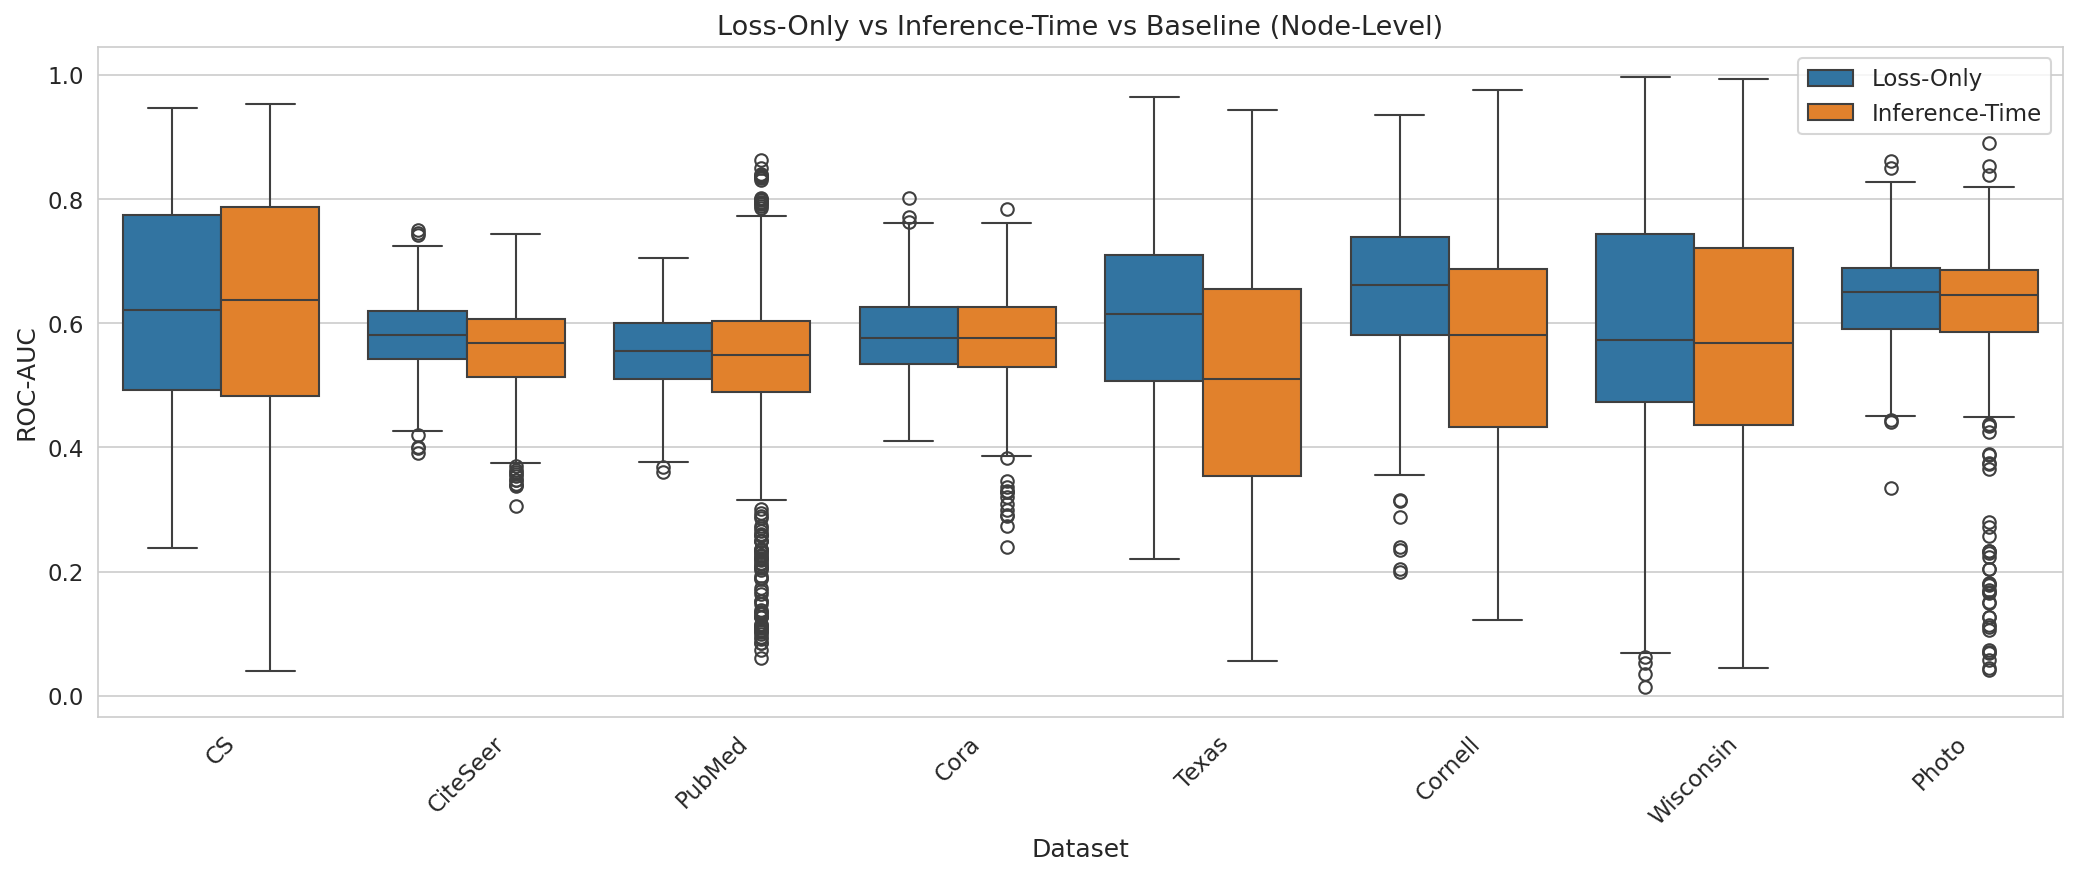
\includegraphics[width=\textwidth]{plots/node_loss_vs_inference.png}
    \caption{ROC-AUC comparison of loss-only and constraint-aware inference models for node-level prediction. Each point represents one hyperparameter configuration.}
    \label{fig:loss_vs_inference_node}
\end{figure}

For node-level prediction, loss-only models achieve nearly identical performance to their baseline counterpart across all configurations except on Texas and Cornell, where loss-only models underperform the baseline. The same pattern holds for graph-level prediction with similar exceptions on AIDS and DHFR (Figure~\ref{fig:loss_vs_inference_graph}).

\begin{figure}[H]
    \centering
    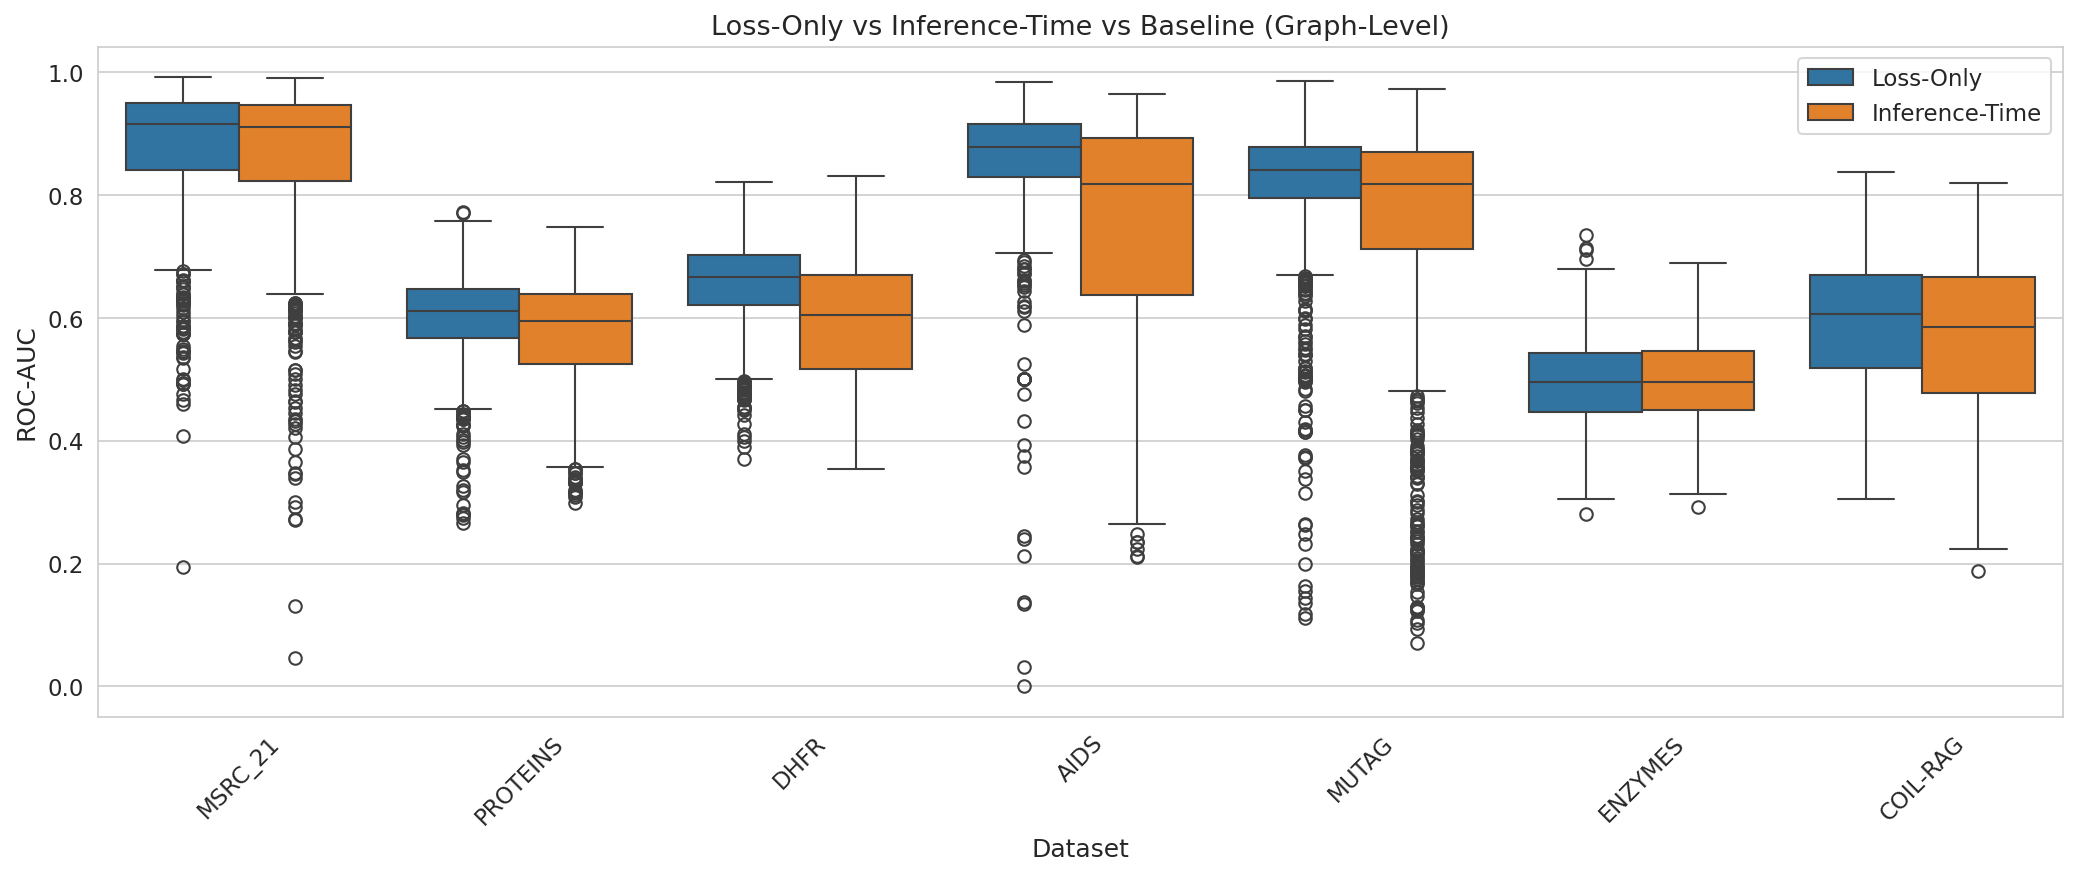
\includegraphics[width=\textwidth]{plots/graph_loss_vs_inference.png}
    \caption{ROC-AUC comparison of loss-only and constraint-aware inference models for graph-level prediction.}
    \label{fig:loss_vs_inference_graph}
\end{figure}

To quantify this, we performed Mann-Whitney U tests comparing loss-only and inference-time models against the baseline separately for node-level and graph-level prediction. For node-level, loss-only models are not significantly different from the baseline ($p = 0.28$), while inference-time models are significantly worse ($p = 0.0009$). The same pattern holds for graph-level: loss-only ($p = 0.92$) and inference-time ($p = 0.005$). In both cases, the difference between loss-only and inference-time is highly significant (node: $p < 10^{-10}$, graph: $p < 10^{-10}$). Disaggregating by variant, Inference-Add is significantly worse than Loss-Add ($p < 10^{-10}$), while Inference-Weighting does not differ from Loss-Weighting ($p = 0.27$). This confirms that the divergence observed in Figure~\ref{fig:loss_vs_inference_node} is systematic: loss-only models preserve baseline performance, while constraint-aware inference—particularly the additive strategy—degrades it on average.

The $\lambda$ sensitivity plots (Figure~\ref{fig:lambda_loss_vs_inference_node}) further illustrate this divergence: loss-only models maintain stable performance across all $\lambda$ values, while constraint-aware models are highly sensitive to the choice of $\lambda$. The same pattern holds at the graph level (Figure~\ref{fig:lambda_loss_vs_inference_graph}).

\begin{figure}[H]
    \centering
    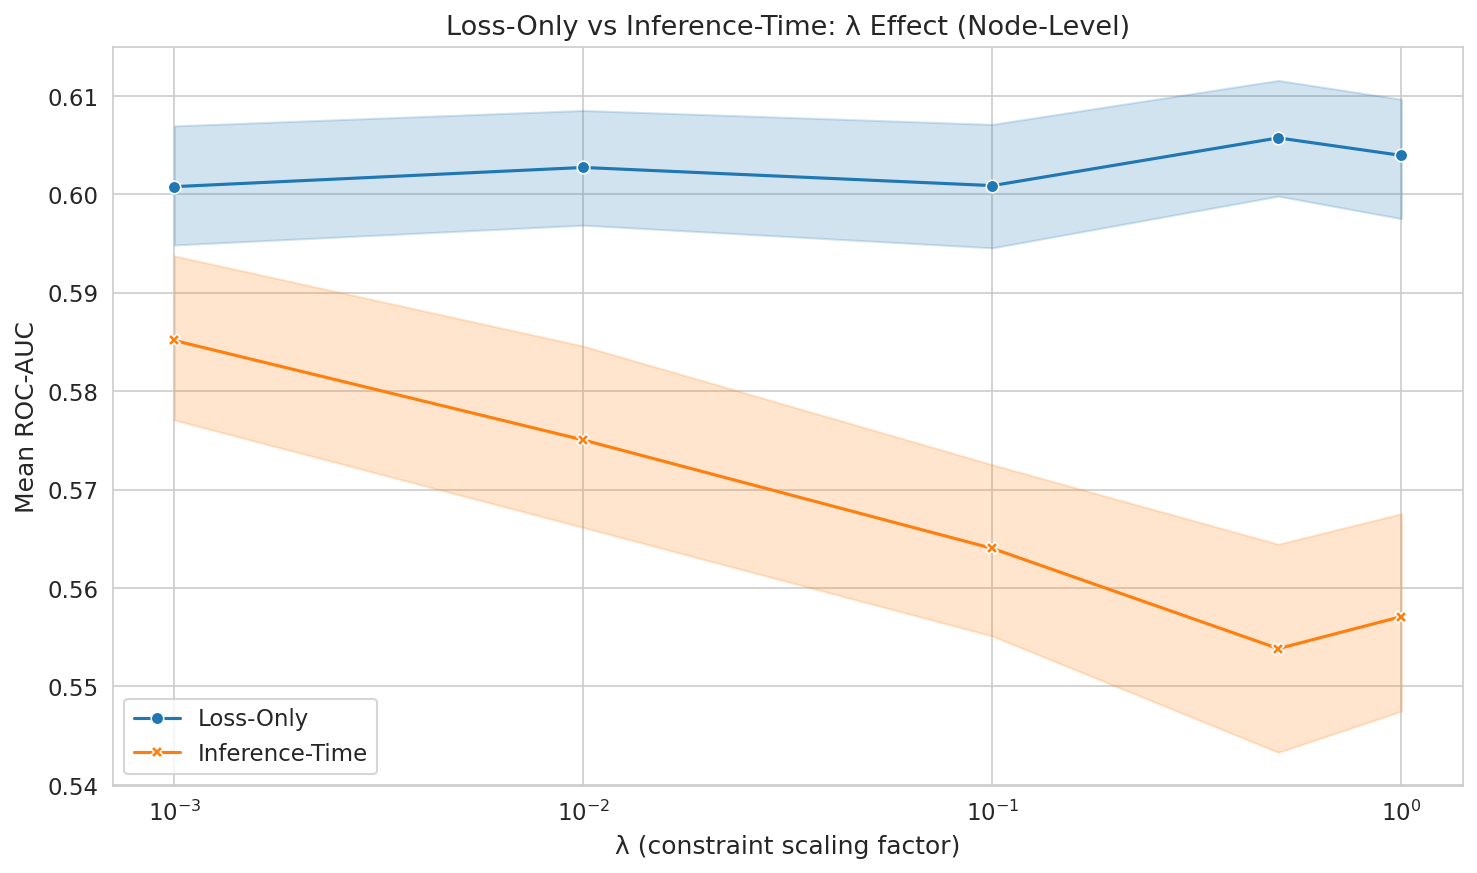
\includegraphics[width=\textwidth]{plots/node_lambda_loss_vs_inference.png}
    \caption{Effect of constraint strength $\lambda$ on ROC-AUC for loss-only and constraint-aware models. Ribbons indicate 95\% confidence intervals.}
    \label{fig:lambda_loss_vs_inference_node}
\end{figure}

\begin{figure}[H]
    \centering
    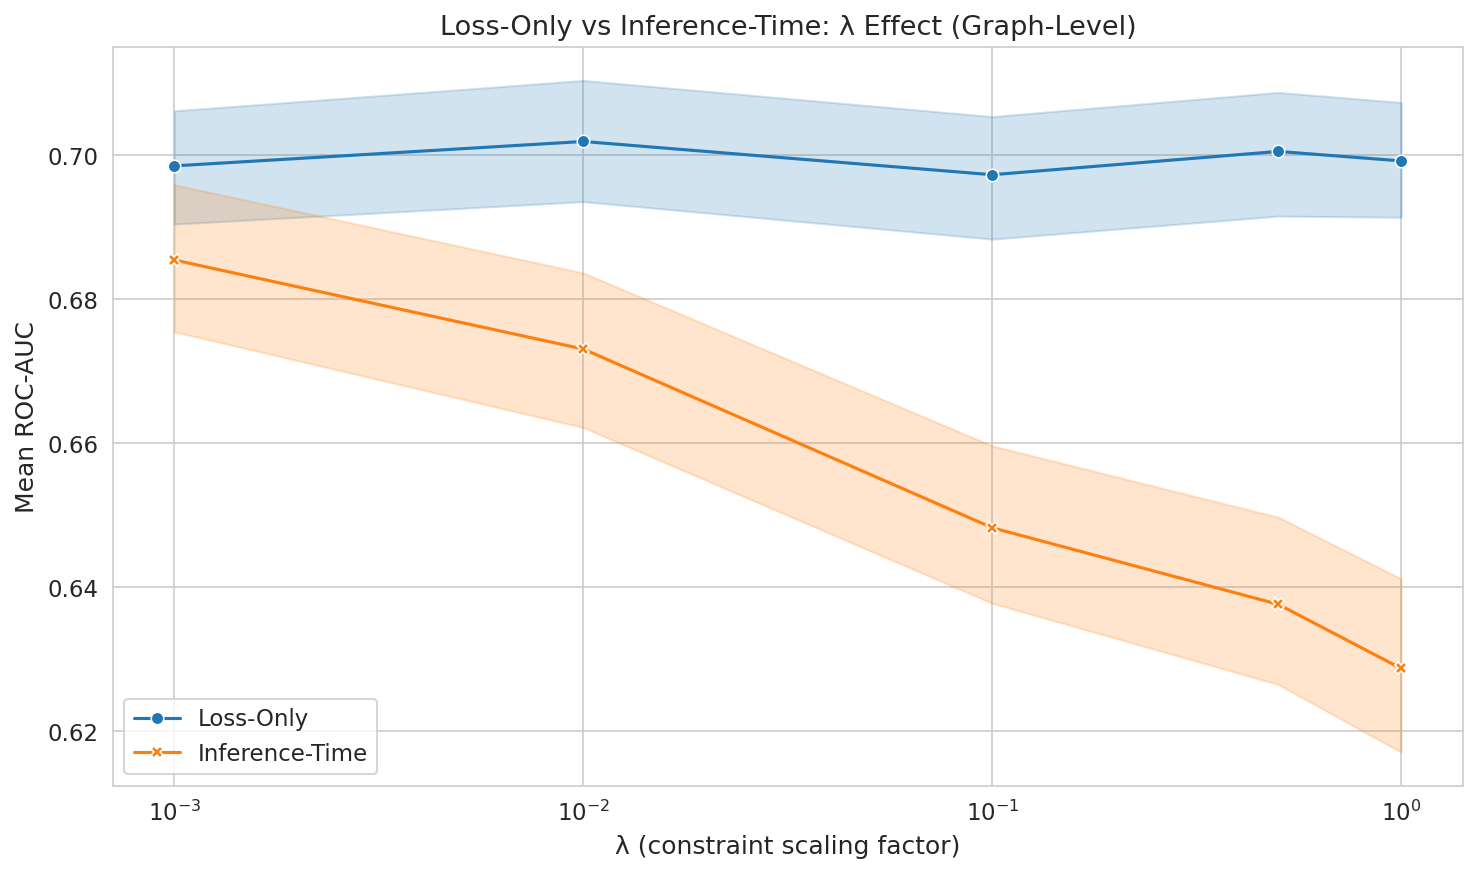
\includegraphics[width=\textwidth]{plots/graph_lambda_loss_vs_inference.png}
    \caption{Effect of $\lambda$ on ROC-AUC for loss-only and constraint-aware models at the graph level.}
    \label{fig:lambda_loss_vs_inference_graph}
\end{figure}

\subsubsection{Constraint Strength Parameter $\lambda$}

Having established that loss-only models preserve baseline performance while inference models degrade it on average (Figure~\ref{fig:loss_vs_inference_node}), we now examine how $\lambda$ modulates this effect. The $\lambda$ hyperparameter controls the weight of the constraint term in the loss function. Figure~\ref{fig:lambda_node} shows how performance varies with $\lambda$ for each model variant.

\begin{figure}[H]
    \centering
    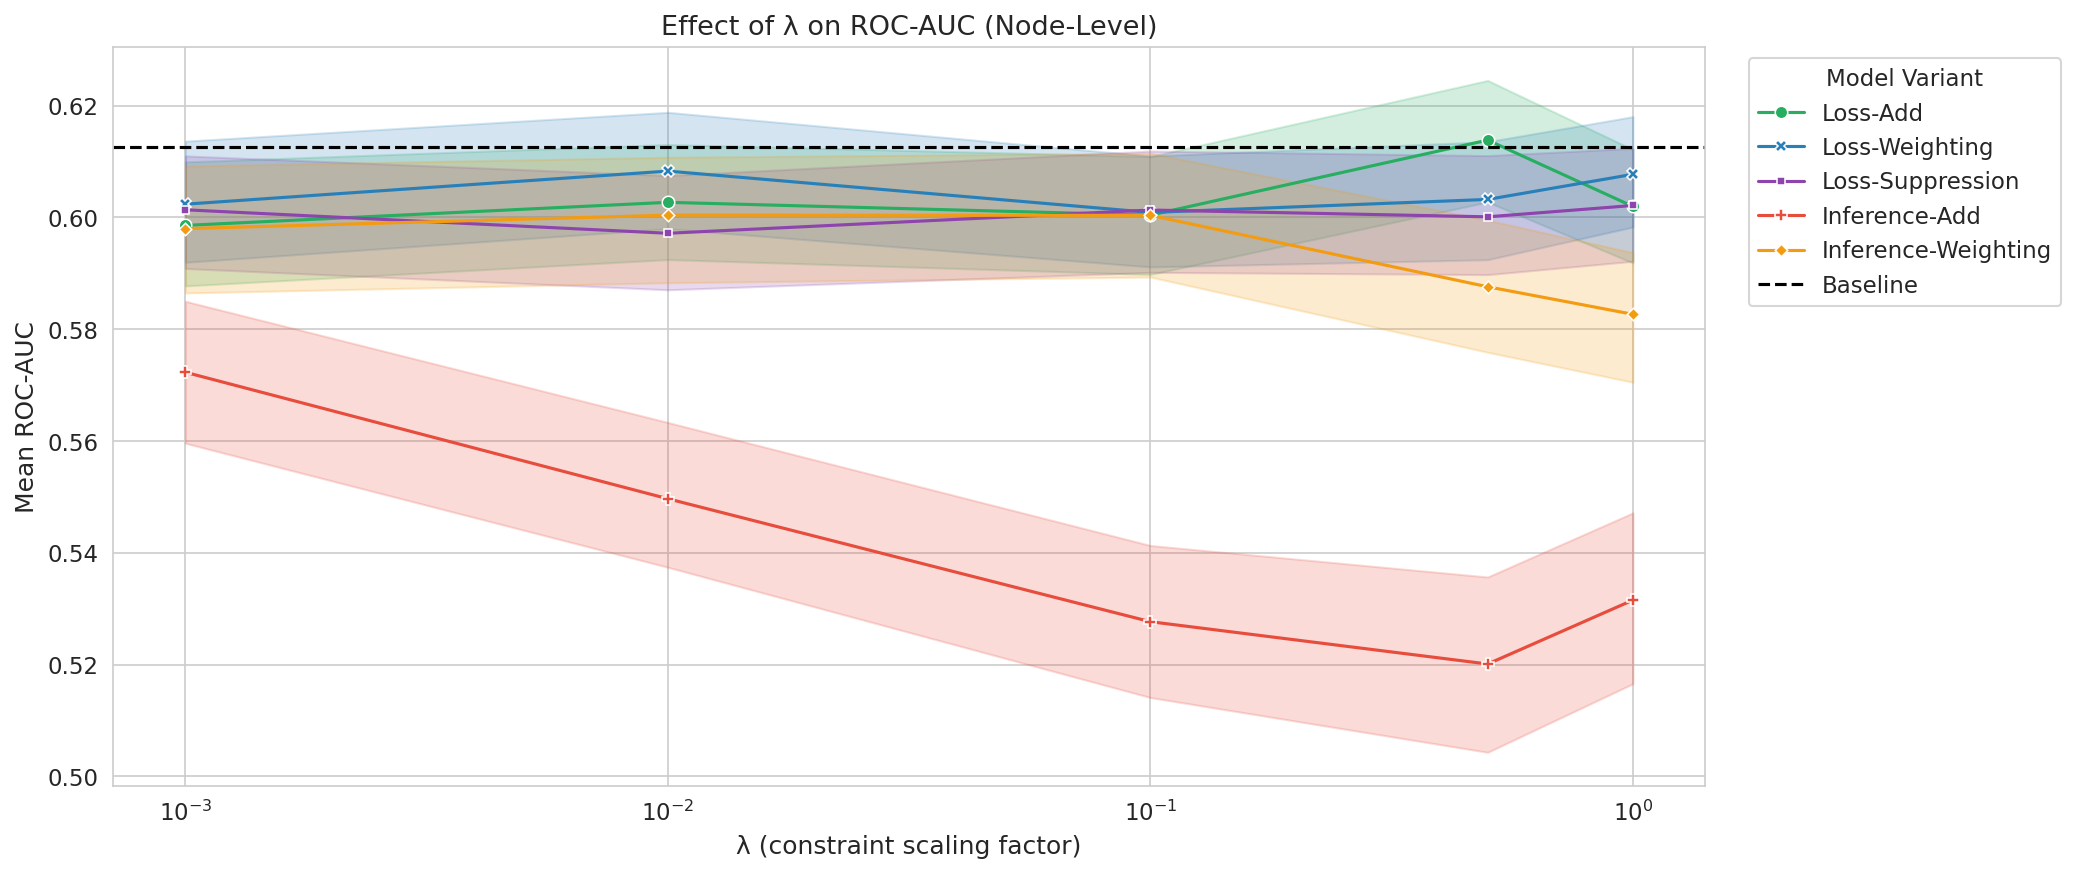
\includegraphics[width=\textwidth]{plots/node_lambda_effect.png}
    \caption{ROC-AUC as a function of $\lambda$ for node-level prediction, faceted by model variant. Confidence bands show 95\% bootstrap intervals.}
    \label{fig:lambda_node}
\end{figure}

For loss-only variants (Loss-Add, Loss-Weighting, Loss-Suppression), $\lambda$ has no systematic effect: performance remains flat across almost the entire range $\lambda \in \{0.001, 0.01, 0.1\}$. At larger values $\{0.5, 1.0\}$, node-level ROC-AUC becomes more variable: it decreases for Inference-Weighting and Loss-Add, but increases for Loss-Suppression and Loss-Weighting. For graph-level, performance is stable across the whole range. In contrast, Inference-Add performance drops sharply even at moderate $\lambda$ values.

\begin{figure}[H]
    \centering
    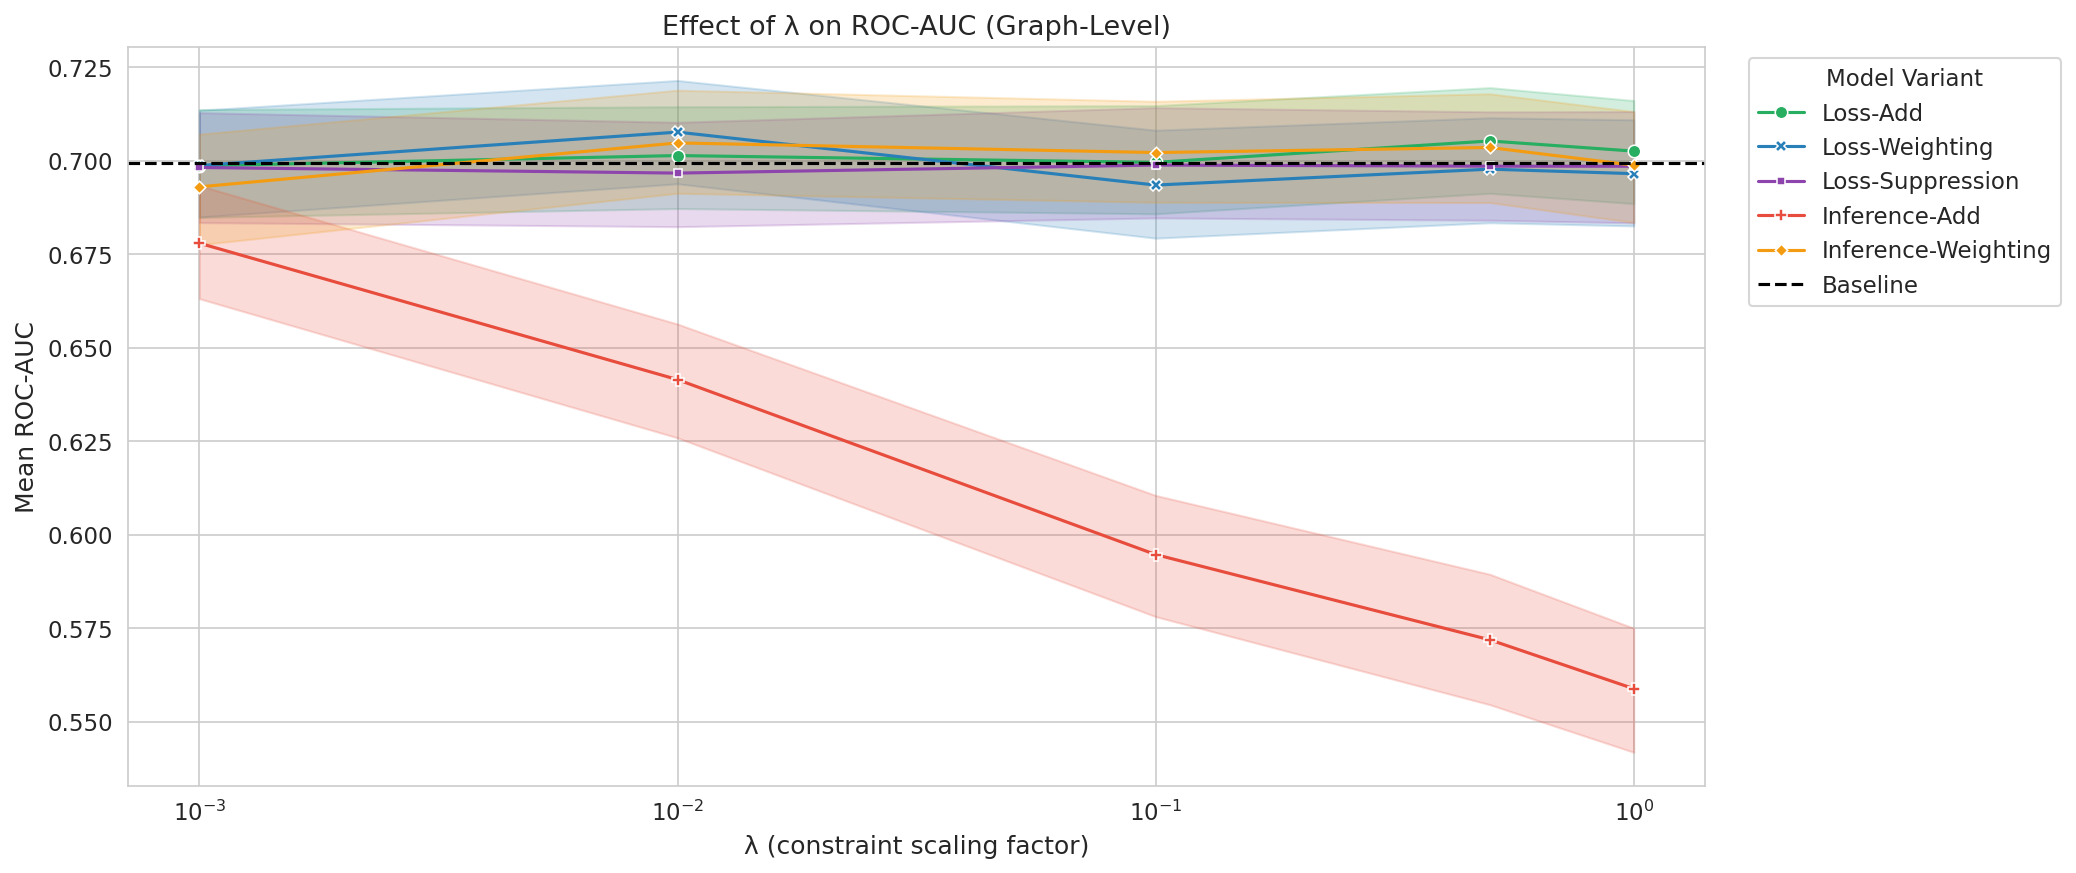
\includegraphics[width=\textwidth]{plots/graph_lambda_effect.png}
    \caption{ROC-AUC as a function of $\lambda$ for graph-level prediction, faceted by model variant.}
    \label{fig:lambda_graph}
\end{figure}

\subsubsection{Handler Comparison}

The constraint evaluation can use either a fuzzy logic handler or a distance-based handler. Figure~\ref{fig:handler_comparison} compares their performance across all model variants.

\begin{figure}[H]
    \centering
    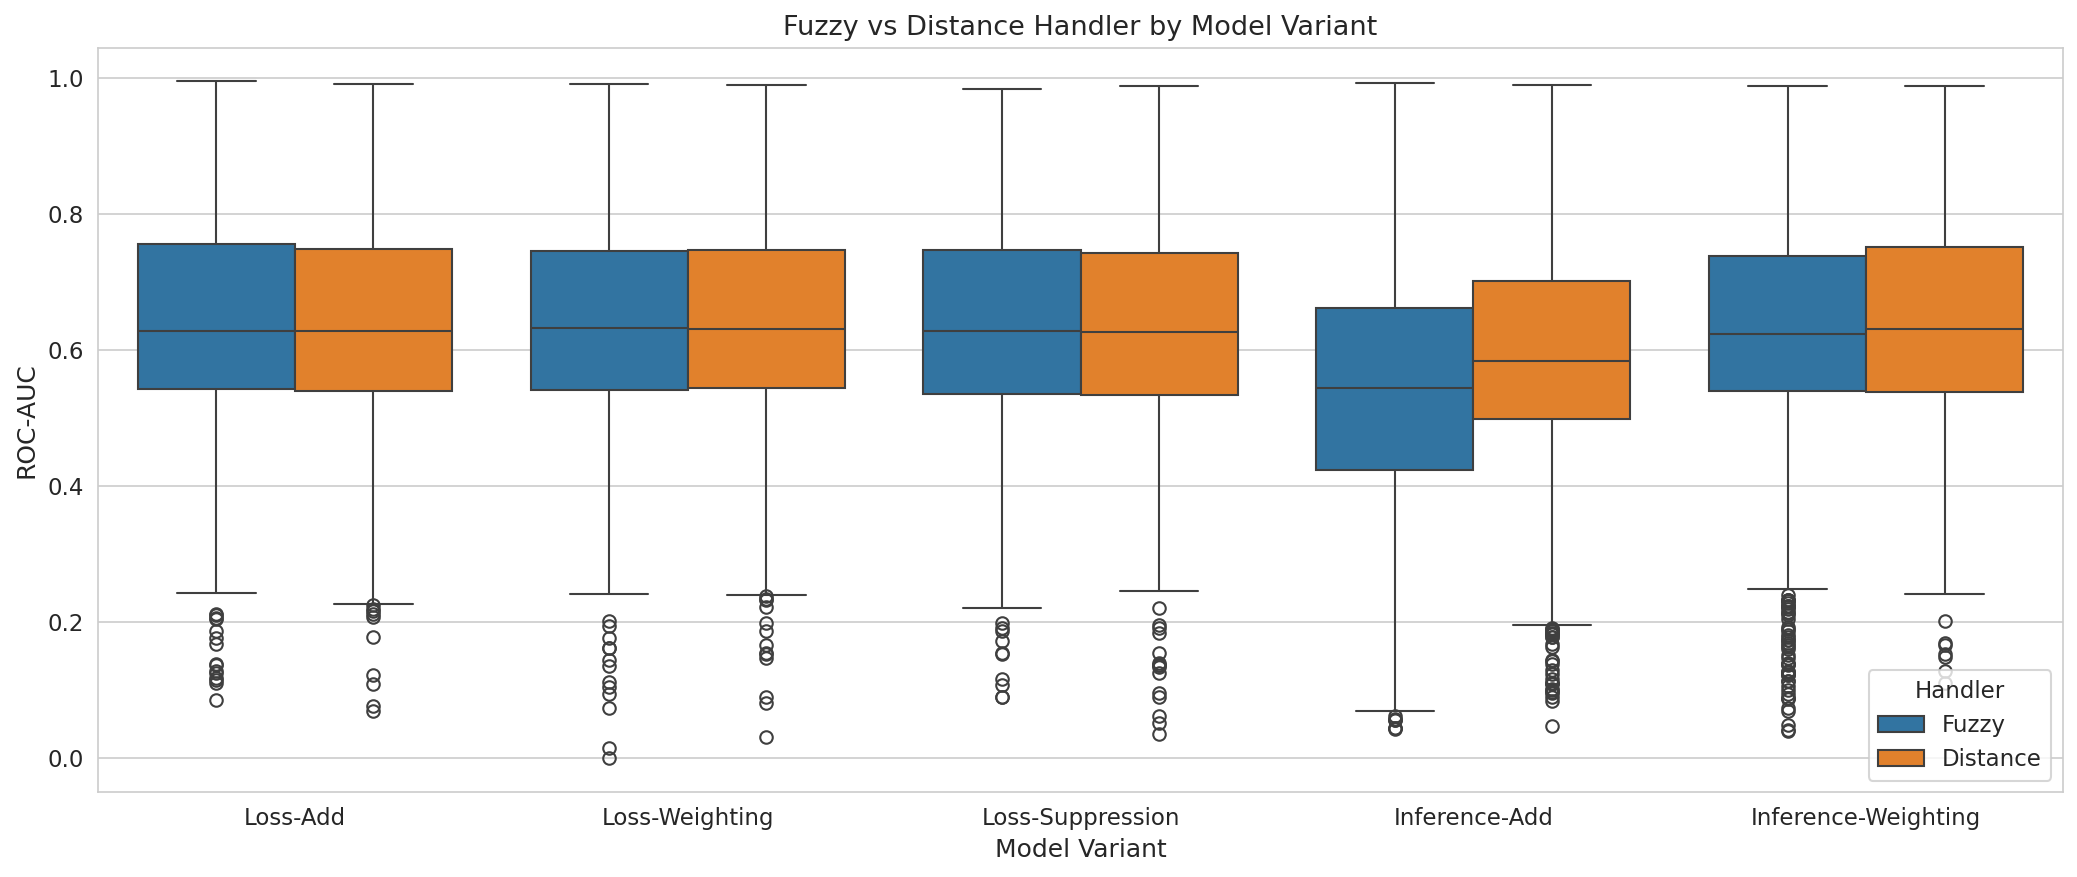
\includegraphics[width=\textwidth]{plots/handler_comparison.png}
    \caption{ROC-AUC comparison of distance-based and fuzzy logic constraint handlers, faceted by model variant.}
    \label{fig:handler_comparison}
\end{figure}

Across most model variants, the distance-based handler consistently outperforms the fuzzy logic handler. A Mann-Whitney U test confirms this difference is highly significant ($p = 1.4 \times 10^{-6}$). The distance-based handler achieves higher median ROC-AUC, especially with the poorly performing Inference-Add strategy.

\subsubsection{Architecture Analysis}

Figure~\ref{fig:architecture_heatmap} shows the effect of hidden dimension and number of layers on model performance.

\begin{figure}[H]
    \centering
    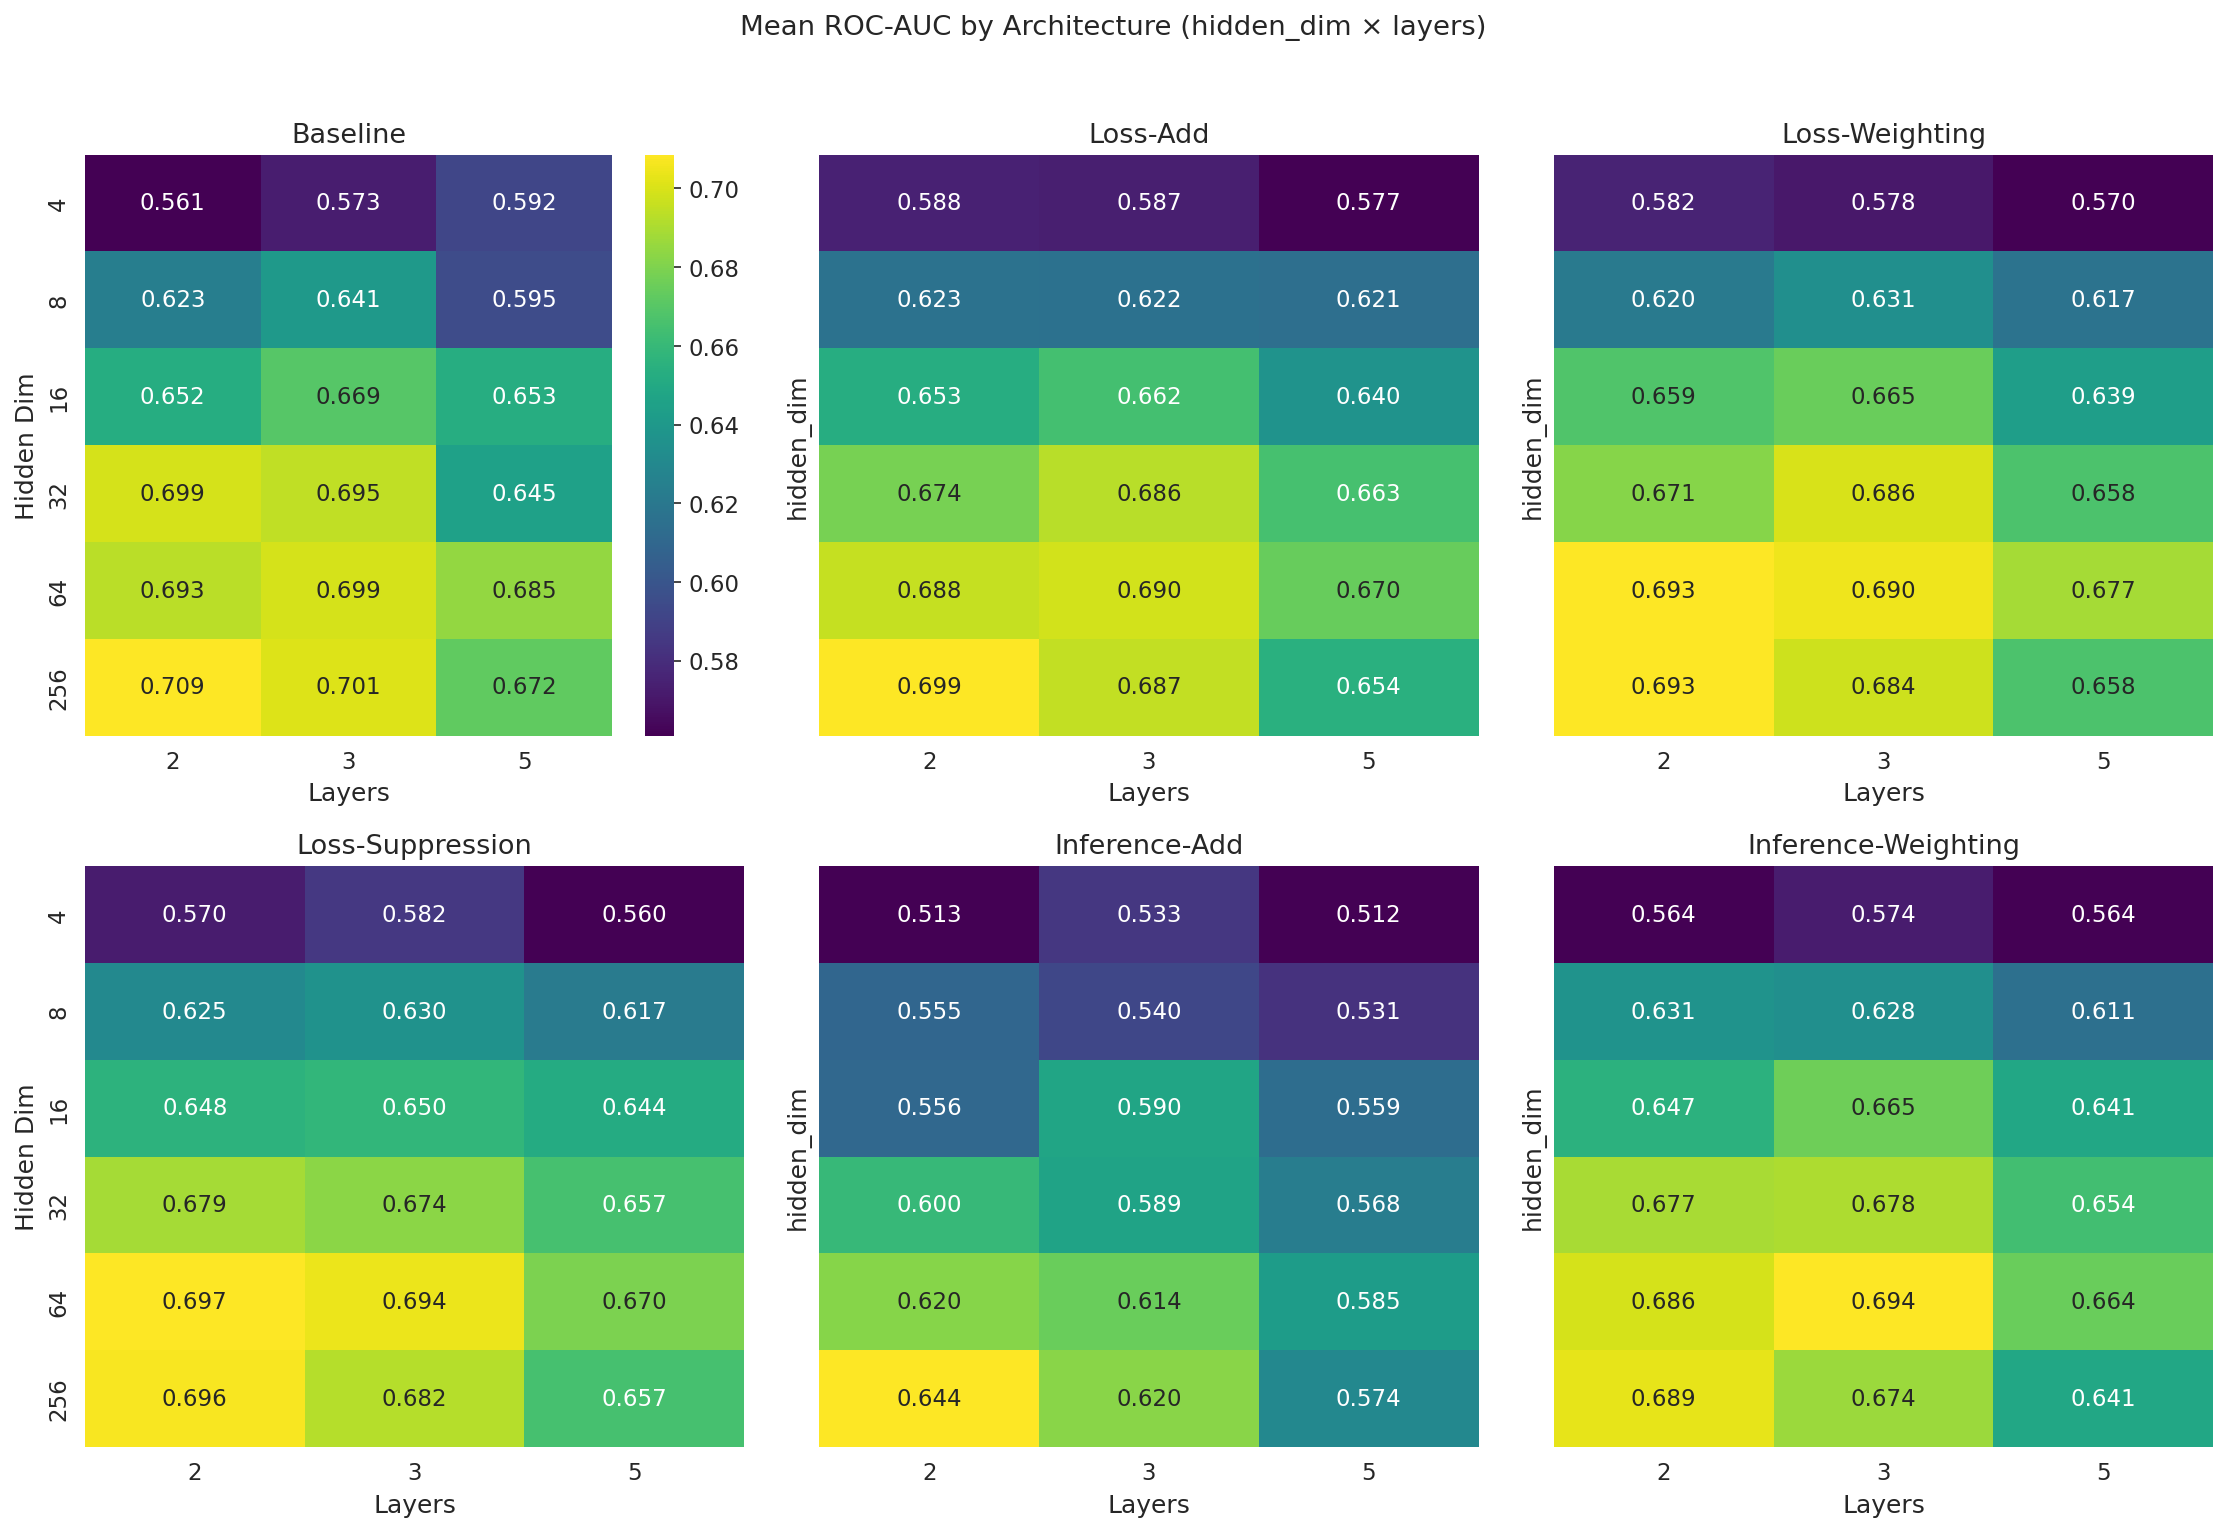
\includegraphics[width=\textwidth]{plots/architecture_heatmap.png}
    \caption{Average ROC-AUC for each combination of hidden dimension and number of layers, faceted by model type.}
    \label{fig:architecture_heatmap}
\end{figure}

The optimal architecture varies by model type. For baseline and loss-only models, moderate hidden dimensions ($d = 16, 32$) with 2--3 layers provide the best trade-off between capacity and generalization. Very small architectures ($d = 4$) lack sufficient capacity, while overly large ones ($d = 256$) show slight degradation. Inference models favor smaller hidden dimensions.

\subsubsection{Best Configurations per Dataset}

Figure~\ref{fig:best_configs} shows the best configuration for each dataset.

\begin{figure}[H]
    \centering
    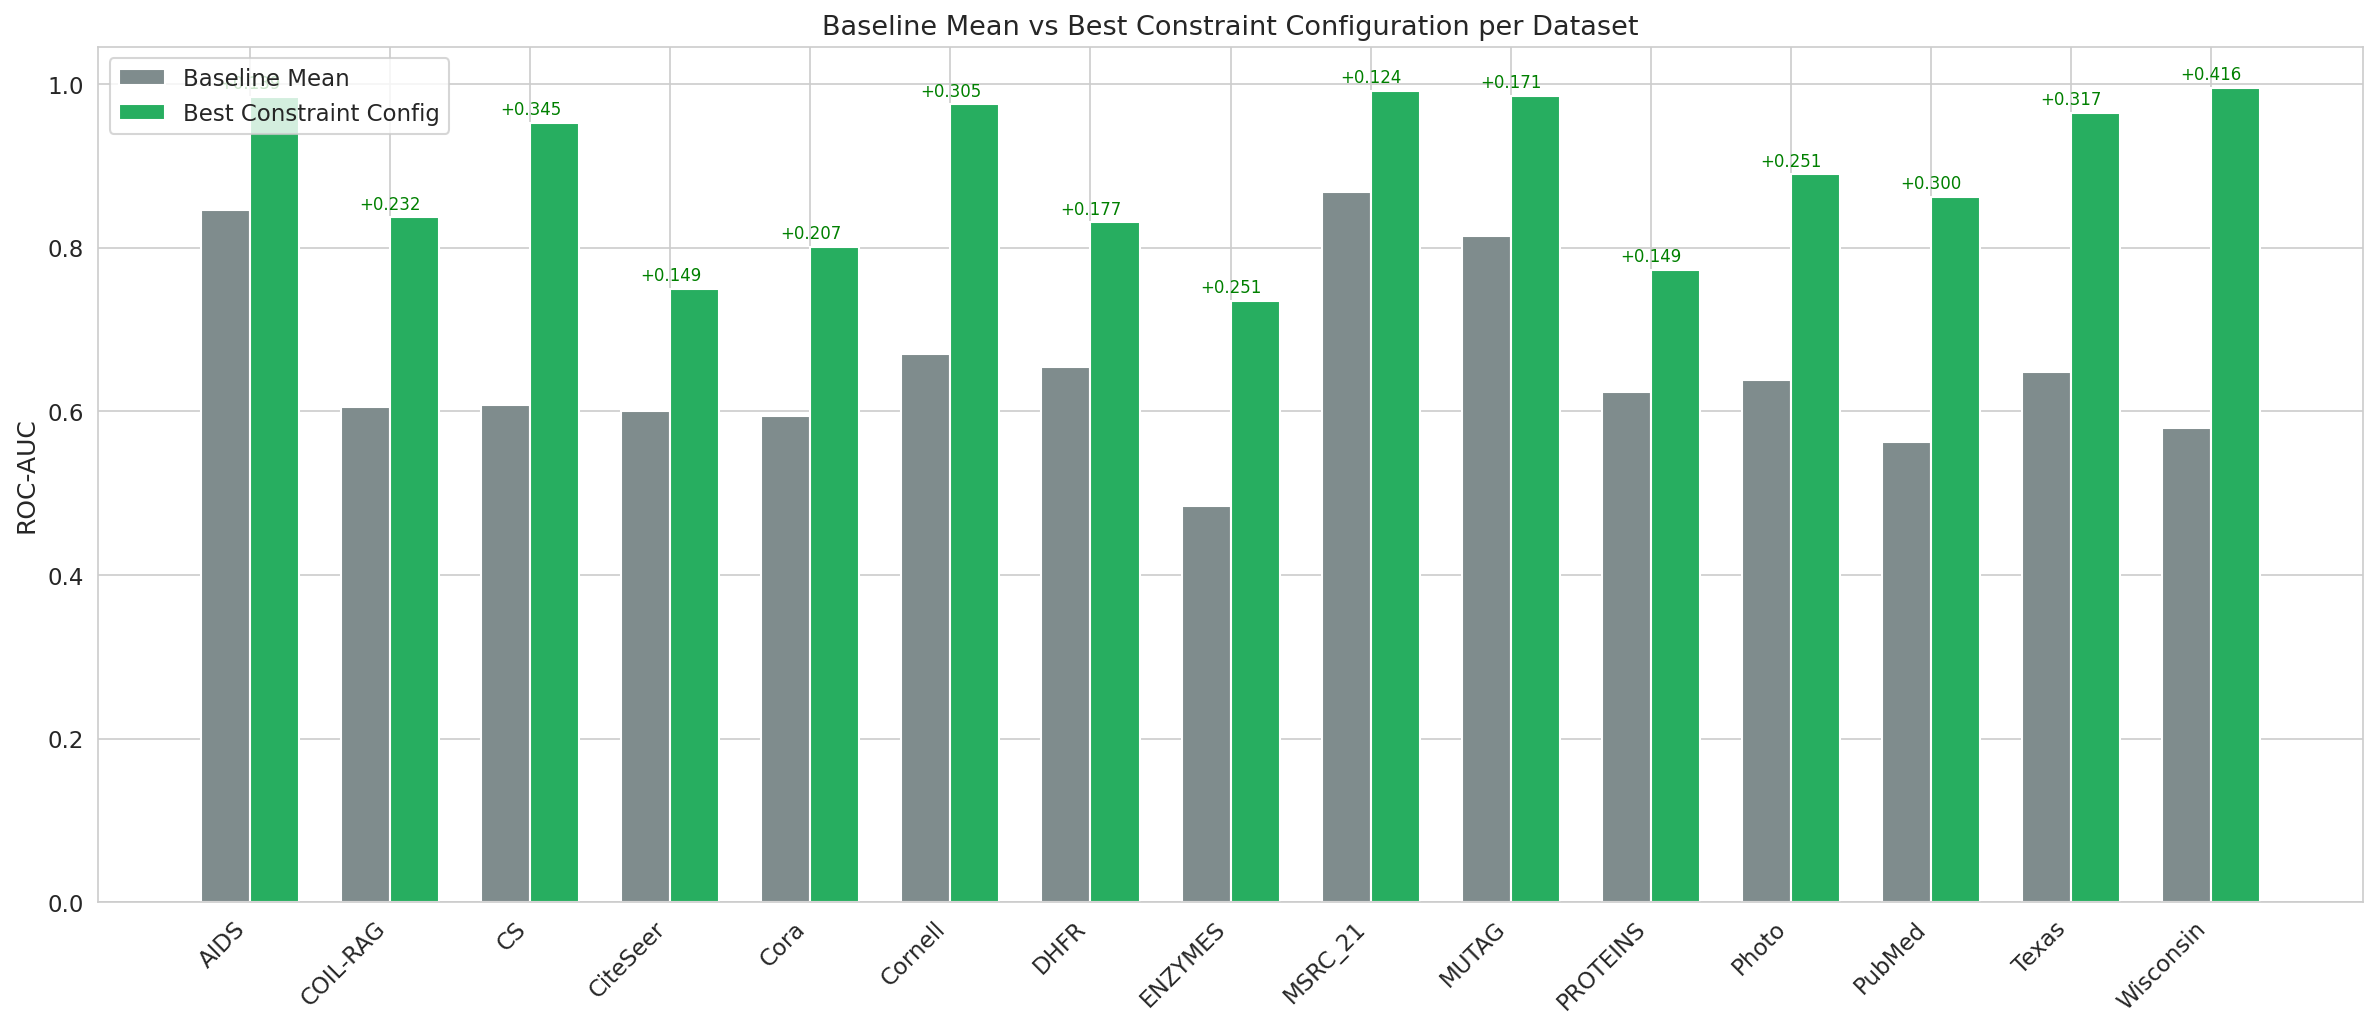
\includegraphics[width=\textwidth]{plots/best_config_highlights.png}
    \caption{ROC-AUC of the best configuration per dataset, grouped by dataset.}
    \label{fig:best_configs}
\end{figure}


A striking finding is that the baseline model never achieves the best performance on any dataset. The best configuration always uses a constraint model---most commonly the distance-based Loss-Add variant with loss-only training. Notably, several of these best configurations use very small $\lambda$ values ($0.001$--$0.1$). The fact that constraint models consistently find superior configurations, despite their average performance matching the baseline, indicates that while the constraint search space includes many poor configurations, it also contains configurations that substantially outperform the baseline.

Tables~\ref{tab:best_configs_node} and~\ref{tab:best_configs_graph} list the exact configurations per dataset. Notably only four of the fifteen best perfoming models used Fuzzy based Handler. Even though on average the Inference-Add strategy perfomed most poorly overall, three of the datasets best configuration used it. Another interesting part is that in eight cases the better performing constraint model needed a two or even four times smaller number of hidden dimentions. four times the dimentions were the same and only on one dataset (Cornell) the best best perfomace was achieved with less number of hidden dimentions. A somewhat similar picture holds for the number of layers.

\begin{table}[H]
\centering
\caption{Best configuration per dataset for node-level prediction. The best ROC-AUC per dataset is bolded.}
\label{tab:best_configs_node}
\begin{tabular}{l l r l r r r}
\toprule
Dataset & Model & ROC-AUC & Handler & Dim & Layers & $\lambda$ \\
\midrule
CS & Baseline & 0.8756 & --- & 256 & 3 & --- \\
   & Inference-Add & \textbf{0.9529} & Fuzzy & 64 & 2 & 1.0 \\
\midrule
CiteSeer & Baseline & 0.6776 & --- & 256 & 2 & --- \\
         & Loss-Add  & \textbf{0.7494} & Distance & 256 & 2 & 0.001 \\
\midrule
Cora & Baseline & 0.6974 & --- & 256 & 2 & --- \\
     & Loss-Weighting  & \textbf{0.8013} & Fuzzy & 64 & 2 & 1.0 \\
\midrule
Cornell & Baseline & 0.8486 & --- & 8 & 3 & --- \\
        & Inference-Add & \textbf{0.9753} & Distance & 16 & 3 & 0.01 \\
\midrule
Photo & Baseline & 0.7510 & --- & 32 & 2 & --- \\
      & Inference-Weighting & \textbf{0.8897} & Distance & 4 & 3 & 0.1 \\
\midrule
PubMed & Baseline & 0.6649 & --- & 64 & 3 & --- \\
       & Inference-Add & \textbf{0.8624} & Distance & 8 & 2 & 1.0 \\
\midrule
Texas & Baseline & 0.8316 & --- & 16 & 5 & --- \\
      & Loss-Add  & \textbf{0.9645} & Distance & 32 & 3 & 0.001 \\
\midrule
Wisconsin & Baseline & 0.9454 & --- & 64 & 3 & --- \\
          & Loss-Add  & \textbf{0.9958} & Fuzzy & 256 & 2 & 0.5 \\
\bottomrule
\end{tabular}
\end{table}

\begin{table}[H]
\centering
\caption{Best configuration per dataset for graph-level prediction. The best ROC-AUC per dataset is bolded.}
\label{tab:best_configs_graph}
\begin{tabular}{l l r l r r r}
\toprule
Dataset & Model & ROC-AUC & Handler & Dim & Layers & $\lambda$ \\
\midrule
AIDS & Baseline & 0.9683 & --- & 64 & 3 & --- \\
     & Loss-Add  & \textbf{0.9845} & Distance & 64 & 2 & 0.001 \\
\midrule
COIL-RAG & Baseline & 0.7518 & --- & 256 & 5 & --- \\
         & Loss-Add  & \textbf{0.8373} & Distance & 32 & 5 & 0.5 \\
\midrule
DHFR & Baseline & 0.7623 & --- & 256 & 2 & --- \\
     & Inference-Add & \textbf{0.8309} & Distance & 64 & 3 & 0.1 \\
\midrule
ENZYMES & Baseline & 0.6171 & --- & 32 & 2 & --- \\
        & Loss-Add  & \textbf{0.7349} & Distance & 16 & 3 & 1.0 \\
\midrule
MSRC\_21 & Baseline & 0.9683 & --- & 32 & 2 & --- \\
         & Loss-Add  & \textbf{0.9916} & Distance & 16 & 2 & 0.1 \\
\midrule
MUTAG & Baseline & 0.9529 & --- & 256 & 2 & --- \\
      & Loss-Suppression  & \textbf{0.9854} & Distance & 256 & 3 & 1.0 \\
\midrule
PROTEINS & Baseline & 0.7408 & --- & 256 & 2 & --- \\
         & Loss-Suppression  & \textbf{0.7730} & Fuzzy & 256 & 2 & 0.01 \\
\bottomrule
\end{tabular}
\end{table}

\clearpage
\section{Conclusion and Outlook}
\label{sec:conclusion}

In this thesis, we investigated the integration of logical constraints into the One Class graph Isomorh Networks. We developed an automatic constraint generation pipeline based on decision trees, evaluated three integration strategies (additive, weighting, suppression), and distinguished between loss-only and constraint-aware inference paradigms.

Our experimental results across 15 datasets and 27,261 individual trials lead to four principal findings. First, loss-only constraint models perform indistinguishably from the baseline OCGIN (Mann-Whitney U test, all $p > 0.28$). Second, constraint-aware inference introduces significant sensitivity to the $\lambda$ hyperparameter: while carefully tuned $\lambda$ values can yield the best per-dataset results, the default choice of high $\lambda$ substantially degrades performance. Third, Inference-Add performs significantly worse than all other models (all $p < 10^{-10}$), while Inference-Weighting does not differ from baseline ($p = 0.38$), suggesting that the additive constraint integration is unsuitable when applied at inference time. Fourth, the distance-based constraint handler consistently outperforms fuzzy logic ($p = 1.4 \times 10^{-6}$), and the best-performing configuration on every dataset uses a constraint model rather than the baseline.



Several directions for future work emerge from this study. Extending the constraint generation pipeline to logic gate networks provides an alternative to decision tree-based rule extraction for datasets with binary or categorical features, though a comprehensive evaluation of this approach remains for future work. The significant handler effect---distance-based consistently outperforming fuzzy logic---suggests that the margin-aware scoring mechanism warrants further investigation. Additionally, exploring adaptive $\lambda$ scheduling or learned constraint weighting could mitigate the sensitivity observed in constraint-aware inference. Finally, evaluating the proposed methods on larger and more diverse graph datasets would strengthen the generality of our conclusions.

\clearpage

\printbibliography




\end{document}
